%% ============================================================
%%  Identifiability, optimal experimental design and closed-loop
%%  control for a stochastic model of meditation dynamics
%%  Manuscript built from the "model paper" pipeline (Q1_pipeline_model.md).
%%  Every number is produced by:  python main.py model all --seed 42 --n-base 256 --profiles
%%  followed by  python main.py model figures  (outputs/paper/model/).
%%  The real-data section (Sec. 4.7, App. on ds001787) follows the
%%  python main.py realdata ... steps and  python main.py realdata paper
%%  (outputs/paper/realdata/, numbers in summary.json).
%%  Author: Dung Vu — Phenikaa University
%%  Compile: pdflatex (x2) from the template_latex/ folder; figures are read
%%  from ../outputs/paper/model/ and ../outputs/paper/realdata/ via \graphicspath.
%%  The previous content of this file (the unified BQI paper) is kept in
%%  bqi_original_unified_backup.tex.
%% ============================================================
\documentclass[12pt,a4paper]{article}

%% ─── Core packages ────────────────────────────────────────────────────────────
\usepackage[T1]{fontenc}
\usepackage[utf8]{inputenc}
\usepackage{mathpazo}   % Palatino font
\usepackage{microtype}

%% ─── Page geometry ────────────────────────────────────────────────────────────
\usepackage[
  a4paper,
  top=2.5cm, bottom=2.5cm,
  left=2.8cm, right=2.8cm,
  headheight=15pt
]{geometry}

%% ─── Math ─────────────────────────────────────────────────────────────────────
\usepackage{amsmath,amssymb,amsfonts,amsthm}
\usepackage{mathtools}
\usepackage{bm}
\usepackage{physics}

%% ─── Algorithms ───────────────────────────────────────────────────────────────
\usepackage[ruled,vlined,linesnumbered]{algorithm2e}
\SetAlgoCaptionSeparator{.}

%% ─── Tables ───────────────────────────────────────────────────────────────────
\usepackage{booktabs}
\usepackage{multirow}
\usepackage{array}
\usepackage{tabularx}
\usepackage{longtable}
\usepackage{xcolor}
\usepackage{colortbl}
\usepackage{makecell}
\usepackage{stackengine}

%% ─── Graphics and plots ───────────────────────────────────────────────────────
\usepackage{graphicx}
\graphicspath{{../outputs/paper/model/}{../outputs/paper/realdata/}{./figures/}}
\usepackage{float}
\usepackage{subcaption}
\usepackage{tikz}
\usepackage{pgfplots}
\pgfplotsset{compat=1.18}
\usetikzlibrary{
  arrows.meta, positioning, shapes.geometric, shapes.multipart,
  backgrounds, fit, calc,
  decorations.markings, matrix, patterns, shadows
}
\usepgfplotslibrary{fillbetween, statistics, groupplots}

%% ─── Code listings ────────────────────────────────────────────────────────────
\usepackage{listings}
\lstset{
  basicstyle=\ttfamily\footnotesize,
  breaklines=true,
  frame=single,
  rulecolor=\color{gray!40},
  backgroundcolor=\color{gray!6},
  keywordstyle=\color{blue!70!black}\bfseries,
  commentstyle=\color{green!50!black}\itshape,
  stringstyle=\color{red!60!black},
  numberstyle=\tiny\color{gray},
  numbers=left,
  stepnumber=1,
  tabsize=2,
  showstringspaces=false,
  xleftmargin=1.5em
}

%% ─── Headers / footers ────────────────────────────────────────────────────────
\usepackage{fancyhdr}
\pagestyle{fancy}
\fancyhf{}
\fancyhead[L]{\small\itshape Identifiability, design and control of a meditation-dynamics model}
\fancyhead[R]{\small\itshape Vu}
\fancyfoot[C]{\small\thepage}
\renewcommand{\headrulewidth}{0.4pt}
\renewcommand{\footrulewidth}{0.4pt}

%% ─── Typography / spacing ─────────────────────────────────────────────────────
\usepackage{setspace}
\setstretch{1.15}
\usepackage{parskip}
\setlength{\parskip}{4pt}
\setlength{\parindent}{1.2em}

%% ─── References ───────────────────────────────────────────────────────────────
\usepackage[numbers,square,sort&compress]{natbib}

%% ─── Hyperlinks ───────────────────────────────────────────────────────────────
\usepackage[
  colorlinks=true,
  linkcolor=blue!60!black,
  citecolor=green!50!black,
  urlcolor=blue!70!black
]{hyperref}
\usepackage{cleveref}

%% ─── Section styling ──────────────────────────────────────────────────────────
\usepackage{titlesec}
\titleformat{\section}{\large\bfseries\color{blue!20!black}}{\thesection.}{0.6em}{}[\vspace{-2pt}\hrule height 0.4pt\vspace{2pt}]
\titleformat{\subsection}{\normalsize\bfseries\color{blue!35!black}}{\thesubsection.}{0.5em}{}
\titleformat{\subsubsection}{\normalsize\itshape\bfseries\color{blue!50!black}}{\thesubsubsection.}{0.4em}{}

%% ─── Theorem environments ─────────────────────────────────────────────────────
\theoremstyle{plain}
\newtheorem{theorem}{Theorem}[section]
\newtheorem{proposition}[theorem]{Proposition}
\newtheorem{lemma}[theorem]{Lemma}
\newtheorem{corollary}[theorem]{Corollary}
\theoremstyle{definition}
\newtheorem{definition}[theorem]{Definition}
\theoremstyle{remark}
\newtheorem{remark}[theorem]{Remark}
\newtheorem{example}[theorem]{Example}

%% ─── Custom colours ───────────────────────────────────────────────────────────
\definecolor{mathbg}{rgb}{0.96,0.97,0.99}
\definecolor{algbg}{rgb}{0.97,0.97,0.97}
\definecolor{hdrcol}{rgb}{0.10,0.22,0.38}
\definecolor{rowA}{rgb}{0.91,0.95,0.98}
\definecolor{rowB}{rgb}{1.00,1.00,1.00}
\definecolor{BQIblue}{RGB}{30,90,160}
\definecolor{BQIgreen}{RGB}{20,140,80}
\definecolor{BQIorange}{RGB}{210,100,20}
\definecolor{BQIred}{RGB}{180,40,40}
\definecolor{BQIgray}{RGB}{90,90,90}
\definecolor{BQIlightblue}{RGB}{200,220,245}
\definecolor{BQIlightgreen}{RGB}{200,240,210}
\definecolor{BQIlightorange}{RGB}{255,230,200}

%% ─── Misc helpers ─────────────────────────────────────────────────────────────
\usepackage{caption}
\captionsetup{font=small,labelfont=bf}
\usepackage{enumitem}
\setlist[itemize]{topsep=2pt,itemsep=1pt}
\setlist[enumerate]{topsep=2pt,itemsep=1pt}
\usepackage{mdframed}
\usepackage{tcolorbox}
\tcbuselibrary{skins,breakable,theorems}

%% ─── tcolorbox styles ─────────────────────────────────────────────────────────
\tcbset{
  mathbox/.style={
    enhanced, breakable,
    colback=mathbg, colframe=blue!30!black,
    boxrule=0.6pt, arc=3pt,
    left=6pt, right=6pt, top=4pt, bottom=4pt,
    fonttitle=\bfseries\small,
    attach boxed title to top left={yshift=-2mm,xshift=4mm},
    boxed title style={colback=blue!15!white,colframe=blue!30!black,arc=2pt,boxrule=0.4pt}
  },
  algbox/.style={
    enhanced, breakable,
    colback=algbg, colframe=gray!50,
    boxrule=0.5pt, arc=2pt,
    left=4pt, right=4pt, top=3pt, bottom=3pt
  },
  notebox/.style={
    enhanced,
    colback=yellow!10, colframe=orange!60!black,
    boxrule=0.5pt, arc=3pt,
    left=6pt, right=6pt, top=3pt, bottom=3pt,
    fonttitle=\bfseries\small\color{orange!60!black},
    attach boxed title to top left={yshift=-2mm,xshift=4mm},
    boxed title style={colback=yellow!15,colframe=orange!60!black,arc=2pt,boxrule=0.4pt}
  }
}

%% ─── Macros ───────────────────────────────────────────────────────────────────
\newcommand{\vF}{\mathcal{F}}
\newcommand{\vS}{\mathcal{S}}
\newcommand{\vH}{\mathcal{H}}
\newcommand{\vB}{\mathcal{B}}
\newcommand{\vQ}{\mathcal{Q}}
\newcommand{\vA}{\mathcal{A}}
\newcommand{\vPhi}{\Phi}
\newcommand{\DMN}{\mathrm{DMN}}
\newcommand{\PCI}{\mathrm{PCI}}
\newcommand{\BQI}{\mathrm{BQI}}
\newcommand{\KL}{\mathrm{KL}}
\newcommand{\E}{\mathbb{E}}
\newcommand{\R}{\mathbb{R}}
\newcommand{\N}{\mathbb{N}}
\newcommand{\C}{\mathbb{C}}
\newcommand{\One}{\mathbf{1}}
\newcommand{\inner}[2]{\left\langle#1,\,#2\right\rangle}
\newcommand{\argmin}{\operatorname*{arg\,min}}
\newcommand{\argmax}{\operatorname*{arg\,max}}
\newcommand{\softmax}{\operatorname{softmax}}
\newcommand{\SNIS}{\mathcal{S}}
\newcommand{\HB}{\mathcal{H}_B}
\newcommand{\PB}{P_B}
\newcommand{\PhiE}{\Phi_E}
\newcommand{\PhiD}{\Phi_D}
\newcommand{\SigmaOp}{\Sigma}
\newcommand{\QoC}{\mathrm{QoC}}
\newcommand{\ADMN}{A_{\mathrm{DMN}}}
% --- macros for this manuscript -------------------------------------------
\newcommand{\kinh}{k_{\mathrm{inh}}}
\newcommand{\kint}{k_{\mathrm{int}}}
\newcommand{\kd}{k_{d}}
\newcommand{\kspont}{k_{\mathrm{spont}}}
\newcommand{\Amax}{A_{\max}}
\newcommand{\sA}{\sigma_{A}}
\newcommand{\sPhi}{\sigma_{\Phi}}
\newcommand{\rA}{r_{A}}
\newcommand{\rPhi}{r_{\Phi}}
\newcommand{\rQ}{r_{Q}}
\newcommand{\CRB}{\mathrm{CRB}}
\newcommand{\RMSE}{\mathrm{RMSE}}
\renewcommand{\dd}{\,\mathrm{d}}   % physics defines \dd; we want a plain differential
\newcommand{\Var}{\operatorname{Var}}
\newcommand{\Cov}{\operatorname{Cov}}
\newcommand{\diag}{\operatorname{diag}}
\newcommand{\thetav}{\boldsymbol{\theta}}
\newcommand{\muv}{\boldsymbol{\mu}}
\newcommand{\xv}{\mathbf{x}}
\newcommand{\yv}{\mathbf{y}}
\newcommand{\hv}{\mathbf{h}}
\newcommand{\uv}{\mathbf{u}}
\newcommand{\code}[1]{\texttt{#1}}

%% ─── Document ─────────────────────────────────────────────────────────────────
\begin{document}

%% ─────────────────────────────────────────────────────────────────────────────
%%  TITLE
%% ─────────────────────────────────────────────────────────────────────────────
\thispagestyle{plain}
\begin{center}
  \vspace{0.4cm}
  {\LARGE\bfseries\color{hdrcol}
    Identifiability, optimal experimental design and\\[4pt]
    closed-loop control for a stochastic model\\[4pt]
    of meditation dynamics
  }

  \vspace{0.8cm}
  {\large Dung Vu$^{1,*}$}

  \vspace{0.3cm}
  {\small
    $^{1}$Phenikaa University, Hanoi, Vietnam\\
    $^{*}$Corresponding author: [institutional e-mail] % TODO: insert before submission
  }

  \vspace{0.3cm}
  {\small\itshape Manuscript draft, \today}
\end{center}

\vspace{0.3cm}
\begin{tcolorbox}[mathbox,title=Abstract]
\small
Dynamical models that link default-mode-network (DMN) activity, information integration ($\Phi$) and a reported ``quality of consciousness'' (QoC) during meditation are increasingly proposed, but three questions that precede any data analysis are rarely asked: whether the model is mathematically consistent, whether its parameters can be identified from the experience-sampling designs actually in use (a few self-report probes per session, sessions of 20--90 minutes, EEG features every few seconds), and what closed-loop control (neurofeedback) can achieve when the parameters are only estimated. We answer all three for a recently proposed three-variable DMN--$\Phi$--QoC model. First, we prove that in the original formulation QoC is a high-pass filter of the derivatives of $\Phi$ and $A_{\mathrm{DMN}}$, so its steady state is identically zero for every parameter value; the closed-form steady states printed with the model do not satisfy its own equations. We propose a linear-Gaussian state-space replacement (M1) with an Ornstein--Uhlenbeck DMN process and an algebraic read-out, and derive its stationary mean, covariance and Gaussian law in closed form. Second, using the exact expected Fisher information of a whole session we characterise structural identifiability for four observation configurations: ratings alone identify 6 of 10 parameters, ratings plus one EEG channel leave one exact scaling symmetry each (made explicit analytically), and ratings with both EEG channels identify all 12 parameters. Over a grid of 144 designs the Cram\'er--Rao bound (CRB) predicts the root-mean-square error of maximum-likelihood recovery within a factor of two in 24 of 24 tested cells (median ratio 0.98), which licenses the CRB as a design tool. The resulting design map shows that the DMN inhibition rate $\kinh$ is the hardest parameter: it needs about eight subject-hours of two-channel EEG (e.g.\ 24 subjects $\times$ 20 min) for a relative error of 20\,\%, whereas $A_0$, $\alpha$ and $\beta$ reach that level with 6 subjects $\times$ 20 min; uniform probe schedules are not beaten by the front-loaded, back-loaded or paired schedules we tested. Third, we recast the control problem as linear-quadratic-Gaussian (LQG) regulation. With true parameters LQG attains a session cost 14 times lower than bang-bang control and 38 times lower than no control, its closed-form stationary cost matches simulation within 3\,\%, and when the controller is designed on parameters estimated from each design the median efficiency loss is a few per cent for designs that meet the identifiability criterion (3\,\% at the reference design) but reaches 38\,\% for the smallest design that fails it (6 subjects, 20-minute sessions). A global Sobol analysis over a $\times 0.25$--$\times 4$ parameter range shows that the identifiability of $\kinh$ is governed by the DMN baseline and its coefficient of variation rather than by $\kinh$ itself. Finally, in a preregistered application to open experience-sampling EEG data (ds001787; 22 of 40 sessions retained after artefact rejection) the Fisher error of $\kinh$ was 10\,\%, within the 9--13\,\% predicted by the design analysis, but the profile likelihood gave 22\,\% and exposed a misspecified alpha-power proxy; the fitted DMN time constant was 0.8~min, and neither EEG proxy improved out-of-sample prediction of the ratings. The simulation results are reproducible from a single command with a fixed seed; EEG features are treated as noisy proxies, and no claim is made about the neural meaning of the parameters.
\end{tcolorbox}

\noindent\textbf{Keywords:} meditation; default mode network; state-space model; Fisher information; structural identifiability; optimal experimental design; experience sampling; Kalman filter; LQG control; neurofeedback; Sobol sensitivity analysis; preregistration; open EEG data.

%% ─────────────────────────────────────────────────────────────────────────────
\section{Introduction}
\label{sec:intro}

Meditation research has moved from describing mean differences between meditators and controls \citep{Brewer2011,Fox2016} towards models of the \emph{dynamics} of a session: the alternation between focused attention, mind wandering and meta-awareness \citep{Hasenkamp2012,Lutz2008,Christoff2016}, the regulation of the default mode network (DMN) \citep{Raichle2001,Brewer2011,Garrison2015}, and theoretical accounts in terms of predictive processing and active inference \citep{Laukkonen2021,SandvedSmith2021}. Several recent proposals go one step further and write explicit differential equations whose state variables are a DMN activity level, a measure of information integration $\Phi$ \citep{Tononi2004,Oizumi2014} and a scalar ``quality of consciousness'' (QoC) that is supposed to be reported by the practitioner. One such model, published as part of a broader framework in \citet{BQI}, is a three-variable ordinary differential equation (ODE) system which we denote M0 and reproduce in \Cref{sec:model}.

Models of this kind are attractive because they connect three streams of data that meditation studies routinely collect: a continuous electrophysiological signal (EEG features every few seconds), occasional self-reports obtained with experience-sampling probes \citep{Hasenkamp2012,Weinstein2018,Brandmeyer2018}, and an experimental manipulation (instruction or feedback). But before such a model can be fitted, three questions must be answered, and to our knowledge none of them has been addressed for any model of meditation dynamics:
\begin{enumerate}[label=(\roman*)]
  \item \textbf{Consistency.} Does the model have the qualitative behaviour it is claimed to have? In particular, does it possess a non-trivial steady state for the reported quantity?
  \item \textbf{Identifiability and design.} Can the parameters be determined from the designs actually in use---$N$ subjects, sessions of 20--90 minutes, probes every 0.5--4 minutes, EEG of a given signal-to-noise ratio---and if so, how many subjects and how long a session are needed for a given precision?
  \item \textbf{Control.} If the model is used to drive a closed loop (neurofeedback, \citealp{Sitaram2017,Ros2020}), what does the loop gain over simple strategies, and how much of that gain survives when the controller is designed on estimated rather than true parameters?
\end{enumerate}
Questions (ii) and (iii) are classical in systems identification and systems biology \citep{Bellman1970,Rothenberg1971,Walter1997,Ljung1999,Raue2009,Chis2011,Villaverde2016,Wieland2021,Kreutz2009}, and (iii) in stochastic control \citep{Astrom1970,Anderson1990}, but their combination has not been applied to the experience-sampling setting, where a latent two-dimensional process is observed through a dense noisy channel (EEG) and a sparse noisy channel (ratings), and where the design variables are the number of subjects, the session length and the probe interval.

\paragraph{Contributions.}
\begin{enumerate}
  \item \textbf{A correction of the original model} (\Cref{sec:model}, \Cref{sec:res-m0}). We prove that in M0 the QoC equation is a first-order high-pass filter acting on $\alpha\dot\Phi-\beta\dot A$, so that $\QoC^*=0$ for all parameter values and all constant drives, and that the steady-state formulas printed with the model violate the model's own equations (Propositions~\ref{prop:p1}--\ref{prop:p3}). We propose a linear-Gaussian state-space model M1 in which the DMN level is an Ornstein--Uhlenbeck process around a baseline $A_0$ and QoC is an algebraic read-out, and give its stationary mean, covariance and Gaussian law in closed form (Propositions~\ref{prop:p4}--\ref{prop:p5}).
  \item \textbf{Identifiability and a quantitative design map} (\Cref{sec:res-ident,sec:res-design}). Because M1 is linear-Gaussian, the joint distribution of all observations of a session is Gaussian with closed-form moments, and the expected Fisher information can be computed \emph{exactly}, without simulation. We use it (a) to establish structural identifiability by Rothenberg's rank criterion for four observation configurations, exhibiting the exact symmetries that make single-EEG-channel designs non-identifiable; (b) to compute Cram\'er--Rao bounds (CRB) over a grid of 144 designs; (c) to validate the CRB against maximum-likelihood (ML) recovery on simulated data at 24 designs; and (d) to derive minimal designs and simple scaling rules for each parameter.
  \item \textbf{Closed-loop control and its dependence on design quality} (\Cref{sec:res-control}). We formulate the control problem as linear-quadratic-Gaussian (LQG) regulation of QoC towards a target, compare it with a bang-bang policy using the same state estimator, give the closed-loop stationary cost in closed form, and quantify the loss of efficiency when the controller is designed on parameter estimates obtained from each experimental design. This links the design map directly to the achievable performance of a model-based neurofeedback loop.
  \item \textbf{Global sensitivity} (\Cref{sec:res-sens}). A variance-based Sobol analysis over a $\times 0.25$--$\times 4$ range around the nominal parameters shows which conclusions are robust and which parameters govern identifiability and control performance.
  \item \textbf{A preregistered test on open data} (\Cref{sec:res-real}). We fit M1 to the experience-sampling EEG dataset on which the reference design is patterned, compare the error predicted by the design analysis with the error achieved, and test out-of-sample prediction of the ratings against null models, under a locked preregistration and verification gates.
\end{enumerate}

\paragraph{What this paper does not claim.} The simulation results use nominal working points, and the real-data application treats EEG features as noisy proxies: we make no claim that posterior alpha power measures DMN activity or that Lempel--Ziv complexity measures $\Phi$, nor about whether meditation ``increases'' $\Phi$ or QoC. The contribution is methodological: a complete, reproducible analysis of what a specific class of models can and cannot deliver \emph{before} data are collected, design recommendations that experimenters can apply directly, and one preregistered test of these recommendations on open data. All simulation results are produced by a single command from the accompanying code with a fixed random seed (\Cref{sec:repro}).

%% ─────────────────────────────────────────────────────────────────────────────
\section{Models}
\label{sec:model}

\subsection{The original model M0}
\label{sec:m0}

The model of \citet[eqs.~52--54]{BQI} describes a session by three scalar variables: the DMN activity $A(t)\in[0,\Amax]$, an integration measure $\Phi(t)\ge 0$ and the quality of consciousness $\QoC(t)$:
\begin{align}
  \dot A    &= -\kinh\,A + \kspont\,\xi(t), \label{eq:m0A}\\
  \dot \Phi &= \kint\Bigl(1-\frac{A}{\Amax}\Bigr) - \kd\,\Phi, \label{eq:m0Phi}\\
  \dot{\QoC} &= \alpha\,\dot\Phi - \beta\,\dot A - \gamma\,\QoC. \label{eq:m0Q}
\end{align}
Here $\kinh$ is the rate at which practice suppresses DMN activity, $\xi(t)$ a spontaneous activation drive treated as a zero-mean Gaussian process (eq.~51 of \citealp{BQI}) of standard deviation $\sigma_\xi$, $\kint$ and $\kd$ the integration and decay rates of $\Phi$, $\alpha,\beta>0$ gains and $\gamma>0$ a relaxation rate. The point values printed with the model (Table~5 of \citealp{BQI}) are $\kinh=0.043$, $\kspont=0.027$, $\kint=0.081$, $\kd=0.034\ \mathrm{min^{-1}}$, $\alpha=2.34$, $\beta=1.87$, $\gamma=0.19\ \mathrm{min^{-1}}$; no values are given for $\Amax$ and $\sigma_\xi$, and we take $\Amax=1$ (the normalised DMN activity used in that paper's figures) and $\sigma_\xi=0.05$. These numbers are used here only to evaluate the printed formulas; none of the estimates, confidence intervals or sample sizes of that table is used as evidence anywhere in this paper. The following closed-form steady states are stated, ``setting $\dot A_{\mathrm{DMN}}=\dot\Phi=\dot{\QoC}=0$'' \citep[eqs.~55--57]{BQI}:
\begin{equation}
\begin{gathered}
  A^*_{\mathrm{p}}=\frac{\kspont}{\kinh}\sqrt{2\pi\sigma_\xi^2},\qquad
  \Phi^*_{\mathrm{p}}=\frac{\kint}{\kd}\Bigl(1-\frac{A^*_{\mathrm{p}}}{\Amax}\Bigr),\\
  \QoC^*_{\mathrm{p}}=\frac{1}{\gamma}\biggl(\alpha\kint\Bigl(\frac{\Amax-A^*_{\mathrm{p}}}{\Amax\,\kd}\Bigr)+\beta\,\frac{\kspont}{\kinh}\sqrt{2\pi\sigma_\xi^2}\biggr).
\end{gathered}
  \label{eq:paperss}
\end{equation}
(The subscript p marks the printed values; the last term of $\QoC^*_{\mathrm p}$ equals $\beta A^*_{\mathrm p}$.)
With the printed parameters, \eqref{eq:paperss} gives $A^*_{\mathrm p}=0.079$, $\Phi^*_{\mathrm p}=2.19$ and $\QoC^*_{\mathrm p}=27.8$ (\Cref{tab:steady}). We now show that \eqref{eq:paperss} cannot be a steady state of \eqref{eq:m0A}--\eqref{eq:m0Q}.

\subsection{What is wrong with M0}
\label{sec:m0wrong}

Let $v(t)=\alpha\Phi(t)-\beta A(t)$ denote the \emph{drive} of the QoC equation. Then \eqref{eq:m0Q} reads $\dot{\QoC}=\dot v-\gamma\QoC$, a first-order linear equation in $\QoC$ forced by the derivative of $v$.

\begin{proposition}[Steady states of M0; P1]
\label{prop:p1}
For any constant drive $\xi(t)\equiv\bar\xi$ (in particular $\bar\xi=0$, the mean of the noise), the unique equilibrium of \eqref{eq:m0A}--\eqref{eq:m0Q} is
\begin{equation}
  A^*=\frac{\kspont\bar\xi}{\kinh},\qquad \Phi^*=\frac{\kint}{\kd}\Bigl(1-\frac{A^*}{\Amax}\Bigr),\qquad \QoC^*=0,
  \label{eq:m0ss}
\end{equation}
for every admissible value of $(\kinh,\kspont,\kint,\kd,\alpha,\beta,\gamma,\Amax)$. With zero-mean noise, $A^*=0$, $\Phi^*=\kint/\kd$.
\end{proposition}

\begin{proposition}[QoC is a high-pass filter of the drive; P2]
\label{prop:p2}
For any absolutely continuous drive $v$ and any $\gamma>0$,
\begin{equation}
  \QoC(t)=e^{-\gamma t}\bigl[\QoC(0)-v(0)\bigr]+v(t)-\gamma\int_0^t e^{-\gamma(t-s)}\,v(s)\dd s .
  \label{eq:qocsol}
\end{equation}
Equivalently, the transfer function from $v$ to $\QoC$ is $H(s)=s/(s+\gamma)$, whose gain at zero frequency is $H(0)=0$ and whose modulus is $|H(j\omega)|=\omega/\sqrt{\omega^2+\gamma^2}$. In particular, if $v(t)\to v_\infty$ then $\QoC(t)\to 0$.
\end{proposition}

\begin{proposition}[The printed steady states violate the model; P3]
\label{prop:p3}
The triple \eqref{eq:paperss} is not an equilibrium of \eqref{eq:m0A}--\eqref{eq:m0Q} for any value of $\bar\xi$: at any point where $\dot A=\dot\Phi=0$ the right-hand side of \eqref{eq:m0Q} equals $-\gamma\QoC$, which is $-\gamma\QoC^*_{\mathrm p}\neq 0$ at \eqref{eq:paperss}. With the printed parameters and $\bar\xi=0$ the residual vector $(\dot A,\dot\Phi,\dot{\QoC})$ at \eqref{eq:paperss} is $(-3.4\times10^{-3},\,0,\,-5.28)$, of norm $5.28$.
\end{proposition}

Proofs are given in \Cref{app:proofs}. The first component of \eqref{eq:paperss} is also inconsistent with the stated noise model: eq.~55 makes $A^*$ proportional to $\sqrt{2\pi\sigma_\xi^2}$, whereas for the zero-mean drive of eq.~51 the equilibrium of \eqref{eq:m0A} is $A^*=0$ (Proposition~\ref{prop:p1}); a positive $A^*$ would require a positive mean drive $\bar\xi$, which is not part of the model. The consequence of Proposition~\ref{prop:p2} is qualitative, not numerical: in M0 the reported quantity is a \emph{transient}. Any constant level of DMN activity and integration, however favourable, produces zero QoC after a few multiples of $1/\gamma$ (\Cref{fig:highpass}a). A model intended to describe a sustained state of consciousness therefore needs QoC to depend on the \emph{levels} of its inputs, not only on their rates of change. The origin of the error in \eqref{eq:paperss} is visible in its third component: since $\alpha\kint(\Amax-A^*_{\mathrm p})/(\Amax\kd)=\alpha\Phi^*_{\mathrm p}$, eq.~57 reads $\QoC^*_{\mathrm p}=(\alpha\Phi^*_{\mathrm p}+\beta A^*_{\mathrm p})/\gamma$, i.e.\ \eqref{eq:m0Q} was solved with the \emph{levels} substituted for the derivatives $\dot\Phi,\dot A$ (and with the sign of the $\beta$ term reversed); the division by $\gamma$ then inflates $\QoC^*$ by an order of magnitude (\Cref{tab:steady}: $(2.34\times2.195+1.87\times0.079)/0.19=27.8$). Notably, the original framework itself does not use \eqref{eq:m0Q} when it needs a value of QoC: its Algorithm~2 (line~21) and its control objective (eq.~69) evaluate QoC as the algebraic read-out $\alpha\Phi-\beta A_{\mathrm{DMN}}+\gamma_0$ \citep{BQI}. The model proposed next adopts exactly this read-out and thereby removes the inconsistency between the equations and the algorithm.

\subsection{The proposed model M1}
\label{sec:m1}

We keep the two mechanistic ingredients of M0---a DMN level that is suppressed by practice and an integration variable that is fed by DMN disengagement---and repair the two defects identified above: the DMN process is given a non-zero baseline $A_0$ so that it has a proper stationary regime, and QoC becomes the static read-out of the state already used in Algorithm~2 of \citet{BQI}, so that it inherits a non-zero stationary level. (The symbol $A_0$ denotes a baseline here, not the initial amplitude of eq.~51 of \citealp{BQI}.) Rates are per minute.
\begin{align}
  \dd A    &= -\kinh\,(A-A_0)\dd t + \sA\dd W_A, \label{eq:m1A}\\
  \dd \Phi &= \Bigl[\kint\Bigl(1-\frac{A}{\Amax}\Bigr)-\kd\,\Phi\Bigr]\dd t + \sPhi\dd W_\Phi, \label{eq:m1Phi}\\
  \QoC     &= \alpha\,\Phi-\beta\,A+\gamma_0, \label{eq:m1Q}
\end{align}
with independent Wiener processes $W_A,W_\Phi$. In state-space form, $\xv=(A,\Phi)^\top$ obeys the linear stochastic differential equation $\dd\xv=(M\xv+\uv)\dd t+G\dd\mathbf W$ with
\begin{equation}
\begin{gathered}
  M=\begin{pmatrix}-\kinh & 0\\ -\kint/\Amax & -\kd\end{pmatrix},\qquad
  \uv=\begin{pmatrix}\kinh A_0\\ \kint\end{pmatrix},\qquad
  G=\diag(\sA,\sPhi),\\
  \QoC=\hv^\top\xv+\gamma_0,\qquad \hv=\begin{pmatrix}-\beta\\ \alpha\end{pmatrix}.
\end{gathered}
  \label{eq:ss}
\end{equation}
$M$ is lower-triangular with eigenvalues $-\kinh,-\kd<0$, so the process is stable and has a unique stationary distribution.

\begin{proposition}[Stationary moments of M1; P4]
\label{prop:p4}
The stationary mean is $\muv=-M^{-1}\uv$, i.e.
\begin{equation}
  A^*=A_0,\qquad \Phi^*=\frac{\kint}{\kd}\Bigl(1-\frac{A_0}{\Amax}\Bigr),\qquad
  \QoC^*=\alpha\Phi^*-\beta A_0+\gamma_0,
  \label{eq:m1ss}
\end{equation}
and the stationary covariance $P$ is the unique solution of the Lyapunov equation $MP+PM^\top+GG^\top=0$,
\begin{equation}
  P_{AA}=\frac{\sA^2}{2\kinh},\qquad
  P_{A\Phi}=-\frac{\kint}{\Amax}\,\frac{P_{AA}}{\kinh+\kd},\qquad
  P_{\Phi\Phi}=\frac{\sPhi^2-2\kint P_{A\Phi}/\Amax}{2\kd}.
  \label{eq:P}
\end{equation}
$\QoC^*$ is non-zero for generic parameters.
\end{proposition}

\begin{proposition}[Stationary law of QoC; P5]
\label{prop:p5}
In the stationary regime $\xv(t)$ is a Gaussian process with mean $\muv$, covariance $P$ and autocovariance $\Cov(\xv(t+\tau),\xv(t))=e^{M\tau}P$ for $\tau\ge 0$. Consequently $\QoC(t)\sim\mathcal N(\QoC^*,\hv^\top P\hv)$ with autocovariance $\hv^\top e^{M\tau}P\hv$.
\end{proposition}

\subsection{Observation model and nominal parameters}
\label{sec:obs}

A session of length $T$ minutes is divided into epochs of $\Delta=10$~s. In every epoch an EEG feature vector is extracted and modelled as a noisy direct observation of the latent state,
\begin{equation}
  \yv_t=\xv_t+\boldsymbol\eta_t,\qquad \boldsymbol\eta_t\sim\mathcal N\bigl(0,\diag(\rA^2,\rPhi^2)\bigr),
  \label{eq:obsEEG}
\end{equation}
and at the probe epochs $t\in\mathcal P$ (every $T_p$ minutes) the practitioner reports a rating,
\begin{equation}
  \mathrm{rating}_t=\QoC_t+\varepsilon_t,\qquad \varepsilon_t\sim\mathcal N(0,\rQ^2).
  \label{eq:obsRating}
\end{equation}
This mirrors the structure of existing experience-sampling meditation data sets such as ds001787 \citep{Brandmeyer2018}, in which EEG is recorded continuously and probes occur every few minutes. The DMN channel $y_A$ would in practice be an EEG proxy of DMN activity (e.g.\ posterior alpha or a source-localised feature) and $y_\Phi$ a complexity or integration measure; the mapping of real features to $(A,\Phi)$ is outside the scope of the design analysis, which asks what could be learned \emph{if} such features existed with noise levels $\rA,\rPhi$; \Cref{sec:res-real} tries two candidate proxies on ds001787. Four observation configurations are considered: (a) ratings only, (b) ratings $+\,y_A$, (c) ratings $+\,y_\Phi$, (d) ratings $+\,y_A+y_\Phi$.

The free parameter vector is
\begin{equation}
  \thetav=(\kinh,A_0,\sA,\kint,\kd,\sPhi,\alpha,\beta,\gamma_0,\rA,\rPhi,\rQ)\in\R^{12},
\end{equation}
with $\Amax=1$ fixed (it sets the unit of $A$). Nominal values (\Cref{tab:nominal}) are a working point, not estimates: $\kint,\kd,\alpha,\beta$ are the point values printed with M0; $\kinh=0.2$ per minute (DMN time constant 5 min) is deliberately larger than the printed $0.043$ per minute (time constant 23 min), because with the latter a session of 20 to 45 minutes would span only one or two DMN time constants and the model would be close to non-stationary over the session; the integration time constant is $1/\kd\approx 29$~min; $A_0=0.6$ places the baseline inside $(0,\Amax)$; the noise intensities give stationary standard deviations $\mathrm{sd}(A)=0.158$, $\mathrm{sd}(\Phi)=0.240$ and $\mathrm{sd}(\QoC)=0.691$ (see \Cref{tab:nominal}). Every conclusion is re-examined on a $\times0.25$--$\times4$ range around this point in \Cref{sec:res-sens}, whose lower end for $\kinh$ ($0.05\ \mathrm{min^{-1}}$) is close to the printed value, and \Cref{sec:limitations} discusses how the design map should be read for slower DMN dynamics.

\begin{table}[t]
\centering\small
\caption{Nominal parameters of M1 (rates per minute) and the derived stationary quantities.}
\label{tab:nominal}
\setlength{\tabcolsep}{4pt}
\begin{tabular}{llll}
\toprule
Parameter & Meaning & Value & Derived quantity \\
\midrule
$\kinh$ & DMN inhibition (relaxation) rate & 0.20 & $1/\kinh = 5$ min \\
$A_0$ & DMN baseline & 0.60 & $A^*=0.60$ \\
$\sA$ & DMN noise intensity & 0.10 & $\mathrm{sd}_\infty(A)=0.158$, $\mathrm{CV}_\infty(A)=0.26$ \\
$\kint$ & $\Phi$ integration rate & 0.081 & \\
$\kd$ & $\Phi$ decay rate & 0.034 & $1/\kd\approx 29$ min, $\Phi^*=0.953$ \\
$\sPhi$ & $\Phi$ noise intensity & 0.05 & $\mathrm{sd}_\infty(\Phi)=0.240$ \\
$\alpha$ & gain $\Phi\to\QoC$ & 2.34 & \\
$\beta$ & gain $A\to\QoC$ & 1.87 & $\QoC^*=1.108$, $\mathrm{sd}_\infty(\QoC)=0.691$ \\
$\gamma_0$ & rating offset & 0 & (0.3 in the structural analysis) \\
$\rA,\rPhi$ & EEG observation noise sd & 0.10 & \\
$\rQ$ & rating noise sd & 0.30 & \\
$\Amax$ & DMN ceiling (fixed) & 1 & \\
$\Delta$ & epoch length & 10 s & \\
\bottomrule
\end{tabular}
\end{table}

%% ─────────────────────────────────────────────────────────────────────────────
\section{Methods}
\label{sec:methods}

\subsection{Exact discretisation}
\label{sec:disc}

Sampling \eqref{eq:ss} at the epoch length $\Delta$ gives the exact linear-Gaussian recursion
\begin{equation}
\begin{gathered}
  \xv_{k+1}=F\xv_k+\mathbf c+\mathbf w_k,\qquad \mathbf w_k\sim\mathcal N(0,Q),\\
  F=e^{M\Delta},\qquad \mathbf c=M^{-1}(F-I)\uv,\qquad Q=\int_0^\Delta e^{Ms}GG^\top e^{M^\top s}\dd s,
\end{gathered}
  \label{eq:disc}
\end{equation}
where $Q$ is computed with Van Loan's matrix-exponential construction \citep{VanLoan1978} (\Cref{app:vanloan}). No Euler approximation is used anywhere; all simulations, likelihoods and Fisher matrices are exact for the continuous-time model. The initial state of every simulated session is drawn from the stationary law $\mathcal N(\muv,P)$, which is also the prior used by the Kalman filter and the Fisher computation.

\subsection{Likelihood and maximum-likelihood estimation}
\label{sec:mle}

For one session the log-likelihood of $\thetav$ is evaluated by the Kalman filter \citep{Kalman1960,Harvey1989,Durbin2012} with sequential scalar updates (one update per observed channel per epoch; \Cref{app:kalman}), which handles the irregular rating channel naturally. Sessions of different subjects are independent, so $N$ subjects contribute additively. Positive parameters ($\kinh,\sA,\kint,\kd,\sPhi,\rA,\rPhi,\rQ$) are estimated on the log scale, $A_0,\alpha,\beta,\gamma_0$ on the linear scale; we write $\thetav$ for this transformed vector throughout. Maximisation uses L-BFGS-B \citep{Byrd1995} with two starting points per fit: the first is the true parameter vector with every positive parameter multiplied by an independent $\exp(\mathcal N(0,0.3^2))$ factor (so that the optimiser never starts at the truth), the second adds $\mathcal N(0,0.3^2)$ noise to every transformed coordinate of the first; the better of the two optima is retained. The Kalman log-likelihood was verified against the direct Gaussian log-likelihood of the stacked observation vector (\Cref{sec:fisher}) to $10^{-11}$.

\subsection{Exact expected Fisher information}
\label{sec:fisher}

Because M1 is linear-Gaussian and stationary, \emph{all} observations of a session form a jointly Gaussian vector $\mathbf Y\sim\mathcal N(\mathbf m(\thetav),\Sigma(\thetav))$ with closed-form moments: with $\Cov(\xv_t,\xv_s)=F^{\,t-s}P$ for $t\ge s$, the covariance of the stacked latent path is a block-Toeplitz matrix, and each observation is a fixed linear functional of one $\xv_t$ plus independent noise (\Cref{app:fisher}). The expected Fisher information matrix for one session is therefore available exactly,
\begin{equation}
  \mathcal I_{ij}(\thetav)=\pdv{\mathbf m^\top}{\theta_i}\,\Sigma^{-1}\,\pdv{\mathbf m}{\theta_j}
  +\frac12\operatorname{tr}\Bigl(\Sigma^{-1}\pdv{\Sigma}{\theta_i}\Sigma^{-1}\pdv{\Sigma}{\theta_j}\Bigr),
  \label{eq:fisher}
\end{equation}
and $N$ identically designed subjects give $N\mathcal I$. Derivatives of $(\mathbf m,\Sigma)$ are central finite differences in the transformed parameters. No Monte Carlo noise enters any bound reported below. The implementation was checked against the Kalman likelihood (agreement $10^{-13}$) and against the empirical covariance of Kalman score vectors over 3{,}000 simulated sessions (agreement within 5\,\%).

\subsection{Structural identifiability}
\label{sec:structural}

By Rothenberg's theorem \citep{Rothenberg1971}, in a regular model a parameter point is locally identifiable if and only if the information matrix is non-singular there; the null space of $\mathcal I$ consists of the parameter directions along which the distribution of the data does not change to first order. We compute $\mathcal I$ for a long, densely probed session (90 min, probes every minute) in each configuration (a)--(d), with $\gamma_0=0.3$ so that no symmetry is masked by a zero value, normalise it to unit diagonal, and declare the directions whose relative eigenvalue is below $10^{-7}$ non-identifiable. Parameters that do not enter the likelihood at all in a configuration (e.g.\ $\rPhi$ when $y_\Phi$ is not recorded) are reported as \emph{absent}. For each null direction one parameter is fixed (``normalised'') at its nominal value, and the CRB of the remaining parameters is computed from the reduced information matrix. The numerically found null directions are compared with the exact symmetries derived in \Cref{app:symmetry}.

\subsection{Practical identifiability}
\label{sec:practical}

For an identifiable configuration the Cram\'er--Rao bound \citep{Rao1945,Cramer1946} on the covariance of any unbiased estimator is $(N\mathcal I)^{-1}$. We report the \emph{relative} CRB: the square root of the diagonal element for log-scale parameters (a relative standard error to first order), and the square root divided by $|\theta|$ for linear-scale parameters; for $\gamma_0=0$ the absolute standard error is given. All 12 parameters are always estimated jointly, so the bound accounts for all correlations among them. Profile likelihoods \citep{Raue2009} are computed for the three rate constants on one simulated data set of the reference design: each parameter is moved over nine points spanning $\pm0.8$ log units around its true value while all other parameters are re-optimised.

\subsection{Design grid and validation of the bound}
\label{sec:grid}

The \emph{reference design}, patterned on ds001787, is $N=12$ subjects, $T=45$~min, $T_p=2$~min, $\rA=\rPhi=0.1$, configuration (d). The design grid crosses $N\in\{6,12,24,48\}$, $T\in\{20,45,90\}$~min, $T_p\in\{0.5,1,2,4\}$~min and EEG noise $r=\rA=\rPhi\in\{0.05,0.1,0.2\}$, i.e.\ 144 cells, in configuration (d); the CRB is computed in every cell. A design is called \emph{adequate} for a parameter when its relative CRB is at most $20\,\%$.

A bound is useful only if it predicts the error actually achieved. In 24 representative cells spanning the grid, five independent data sets were simulated per cell (seeds a deterministic function of the cell and replicate index), each fitted by ML as in \Cref{sec:mle}, and the root-mean-square error (RMSE) over the five fits computed \emph{in the same scale as the bound} (log for positive parameters, relative for linear ones). Gate M1 of the analysis is passed when, in at least 80\,\% of the cells, at least half of the four key parameters $(\kinh,A_0,\alpha,\beta)$ have $\RMSE/\CRB\in[1/2,2]$. The 24 cells cost about seven hours on a four-core machine and are the only computationally expensive part of the study.

\subsection{Probe schedules}
\label{sec:schedules}

Holding the number of probes fixed (22 probes in a 45-min session), we ask whether a non-uniform schedule reduces the Ds-optimality criterion \citep{Pukelsheim1993,Atkinson2007} $\log\det\bigl[(\mathcal I^{-1})_{\mathcal K\mathcal K}\bigr]$, the log-volume of the confidence ellipsoid of the key parameters $\mathcal K=(\kinh,A_0,\alpha,\beta)$ with all 12 parameters estimated. Two interpretable families are compared with the uniform schedule: power spacing $t_k=T\,((k+\tfrac12)/n)^p$ with $p\in[0.4,2.5]$ (15 values; $p<1$ front-loads, $p>1$ back-loads, $p=1$ is uniform) and paired probes ($n/2$ pairs, partner $g\in\{1,2,3,6,12\}$ epochs later, which inform fast time constants). Efficiency relative to uniform is $\exp[-(\log\det_{\mathrm{opt}}-\log\det_{\mathrm{unif}})/|\mathcal K|]$, the ratio of geometric-mean standard errors.

\subsection{Closed-loop control}
\label{sec:control-methods}

\paragraph{Controlled model.} An intervention $u(t)$ (instruction, feedback, stimulation) is assumed to act on the DMN equation, $\dd A=[-\kinh(A-A_0)-b\,u]\dd t+\sA\dd W_A$ with $b=1$, bounded by $|u|\le u_{\max}=2$. Exact zero-order-hold discretisation gives the input matrix $B=M^{-1}(F-I)\mathbf b$, $\mathbf b=(-b,0)^\top$. The controller observes the EEG channels \eqref{eq:obsEEG} every epoch; ratings are not used for control.

\paragraph{LQG regulator.} The target $\QoC_{\mathrm{tgt}}=2.0$ (about $1.3$ stationary standard deviations above $\QoC^*$) is reached at the unique equilibrium $(\xv_{\mathrm{ss}},u_{\mathrm{ss}})$ with $F\xv_{\mathrm{ss}}+\mathbf c+Bu_{\mathrm{ss}}=\xv_{\mathrm{ss}}$ and $\hv^\top\xv_{\mathrm{ss}}+\gamma_0=\QoC_{\mathrm{tgt}}$. On the deviations the quadratic cost $\sum_t[(\QoC_t-\QoC_{\mathrm{tgt}})^2+\lambda u_t^2]$, $\lambda=0.1$, is minimised by the certainty-equivalence LQG controller \citep{Astrom1970,Anderson1990}: $u_t=u_{\mathrm{ss}}-K(\hat\xv_t-\xv_{\mathrm{ss}})$ with the discrete-time LQR gain $K$ (algebraic Riccati equation with state weight $\hv\hv^\top$) and $\hat\xv_t$ from the stationary Kalman filter for $\yv_t=\xv_t+\boldsymbol\eta_t$; $u_t$ is clipped to $[-u_{\max},u_{\max}]$. For the nominal model $K=(-3.61,\,4.60)$, $\xv_{\mathrm{ss}}=(0.480,1.238)$ and $u_{\mathrm{ss}}=0.024$.

\paragraph{Relation to the original control formulation.} \citet{BQI} states the control task in two ways: Algorithm~2 (line~5) applies proportional feedback $u_{\mathrm{stim}}\leftarrow K\,(\QoC_{\mathrm{target}}-\QoC(t))$ towards a target, while Sec.~9.4 and 10.1 (eqs.~69--75) maximise the terminal or discounted value of QoC subject to the ODE, a bound $\|u_t\|\le\epsilon$ and non-negativity, and conclude from Pontryagin's principle that the optimal stimulation is bang-bang, $u^*=\epsilon\,\mathrm{sign}(\lambda_A)$. Two points in that formulation need repair before any controller can be derived. First, the control variable does not appear in the constraint dynamics (eqs.~70--71 are the uncontrolled ODE), so the stated problem has no channel through which $u$ acts; the controlled model above supplies one by letting $u$ enter the DMN equation with gain $b$. Second, the problem is called linear-quadratic although its objective (eq.~69) is linear in the state and the input is unpenalised; for such a problem the Pontryagin solution is indeed bang-bang, but as soon as the objective is quadratic (hold QoC near a target at moderate effort), the optimal policy is linear feedback on the state estimate, i.e.\ LQG. The LQG formulation above is therefore the stochastic, state-estimated version of the target-tracking reading of Algorithm~2 with the feedback gain chosen optimally rather than set by hand, whereas the bang-bang law is the solution of the linear-objective reading.

\paragraph{Comparators.} \emph{Bang-bang}: $u_t=\pm u_{\max}$ according to the sign of $\QoC_{\mathrm{tgt}}-(\hv^\top\hat\xv_t+\gamma_0)$, using the \emph{same} Kalman estimate, so that the comparison isolates the control law from the estimator. \emph{No control}: $u\equiv0$. Because the bang-bang law solves a different problem, we report, besides the quadratic cost, the two neutral components: tracking mean-squared error $\overline{(\QoC_t-\QoC_{\mathrm{tgt}})^2}$ and the root-mean-square input. All policies are run on the true model over 270 epochs (45 min) with common random numbers, 20 trials.

\paragraph{Closed-form stationary cost.} For the unclipped LQG loop the augmented state $(\xv_t,\hat\xv_t)$ is a linear Gaussian recursion whose stationary mean and covariance follow from a $4\times4$ discrete Lyapunov equation (\Cref{app:lqg}); the stationary cost is then explicit. Gate M2 requires that LQG with true parameters beats both comparators and that this closed form agrees within 20\,\% with a long simulation (4{,}000 epochs, 1{,}000 discarded). The closed form is what the sensitivity analysis evaluates.

\paragraph{Robustness to estimation error.} For each of the 24 validated design cells and each of its five ML fits, an LQG controller (gain \emph{and} filter) is designed on the \emph{estimated} parameters and run on the true model of that cell (nominal parameters with the cell's EEG noise level) for 10 trials; the efficiency loss is $(\mathrm{cost}_{\mathrm{est}}-\mathrm{cost}_{\mathrm{true}})/\mathrm{cost}_{\mathrm{true}}$. We report the median and 90th percentile over fits.

\subsection{Global sensitivity analysis}
\label{sec:sobol-methods}

First-order ($S_1$, Saltelli estimator) and total-order ($S_T$, Jansen estimator) Sobol indices \citep{Sobol1993,Jansen1999,Saltelli2010} are computed for eight inputs, $(\kinh,A_0,\mathrm{CV}_A,\kint,\kd,\sPhi,\alpha,\beta)$, each log-uniform on $[\tfrac14,4]\times$nominal, except that the DMN noise is parametrised by its stationary coefficient of variation $\mathrm{CV}_A=\sA/(A_0\sqrt{2\kinh})\in[0.05,0.4]$ rather than by $\sA$: varying $\sA$ independently drives $A$ below zero for a substantial fraction of the time at the corners of the box (30\,\% at $\sA\times4$, $\kinh\times\tfrac14$), whereas $\mathrm{CV}_A\le0.4$ keeps $\Pr(A<0)\le0.6\,\%$. Four deterministic outputs are analysed: $\QoC^*$; $\Var_\infty(\QoC)=\hv^\top P\hv$; the relative CRB of $\kinh$ at the reference design; and the LQG efficiency, the ratio of the closed-form stationary LQG cost to the cost without control. The last three are positive and vary over orders of magnitude across the box, so they are analysed on the log scale (on the raw scale a handful of extreme samples dominate the variance, indices clip at 1 and $S_1\ll S_T$ spuriously); $\QoC^*$ can change sign and stays on the raw scale. The Saltelli matrices are built from a scrambled Sobol sequence \citep{Owen1998} with base size $n=256$, i.e.\ $n(8+2)=2{,}560$ model evaluations. Ninety-five per cent confidence intervals are obtained by bootstrapping the rows ($B=1{,}000$), and convergence is checked by recomputing $S_T$ from the first half of the sample.

\subsection{Reproducibility and verification gates}
\label{sec:repro}

Every setting above lives in one configuration module; a snapshot is written next to every result. The analysis is organised as five packages with three machine-checked gates: M0 (Propositions~\ref{prop:p1}--\ref{prop:p5} verified numerically on the actual ODE and SDE, not on the formulas: equilibrium and Lyapunov residuals below $10^{-6}$, DC attenuation of the step response above $10^{4}$, sinusoidal amplitude errors below $1\,\%$, Kolmogorov--Smirnov $p>0.01$ on thinned samples), M1 (CRB predicts ML error, \Cref{sec:grid}) and M2 (control, \Cref{sec:control-methods}). All numbers, tables and figures in this paper are produced from seed 42 by
\begin{center}\small\ttfamily
python main.py model all -{}-seed 42 -{}-n-base 256 -{}-profiles\\
python main.py gates
\end{center}
followed by the figure script; 104 unit tests cover the model, filter, Fisher matrix, gates, real-data pipeline and figure scripts. Four further gates (E0--E3) govern the real-data analysis of \Cref{sec:res-real} and are listed there. Computations use NumPy and SciPy \citep{Harris2020,Virtanen2020}. Code and outputs will be archived with a DOI at publication.

%% ─────────────────────────────────────────────────────────────────────────────
\section{Results}
\label{sec:results}

\subsection{The original model has no sustained QoC; the proposed model does}
\label{sec:res-m0}

\begin{table}[t]
\centering\small
\caption{Steady states of the DMN--$\Phi$--QoC model with the parameters printed in \citet{BQI}. ``M0, corrected'' is the equilibrium \eqref{eq:m0ss} with zero-mean noise; ``M1'' is \eqref{eq:m1ss} at the nominal parameters of \Cref{tab:nominal}.}
\label{tab:steady}
\begin{tabular}{lrrr}
\toprule
 & Printed, eqs.~(55)--(57) of \citep{BQI} & M0, corrected (Prop.~\ref{prop:p1}) & M1 (Prop.~\ref{prop:p4}) \\
\midrule
$A^*$            & 0.0787  & 0      & 0.600 \\
$\Phi^*$         & 2.195   & 2.382  & 0.953 \\
$\QoC^*$         & 27.81   & 0      & 1.108 \\
$\Var_\infty(\QoC)$ & --   & --     & 0.477 \\
\bottomrule
\end{tabular}
\end{table}

\begin{figure}[t]
\centering
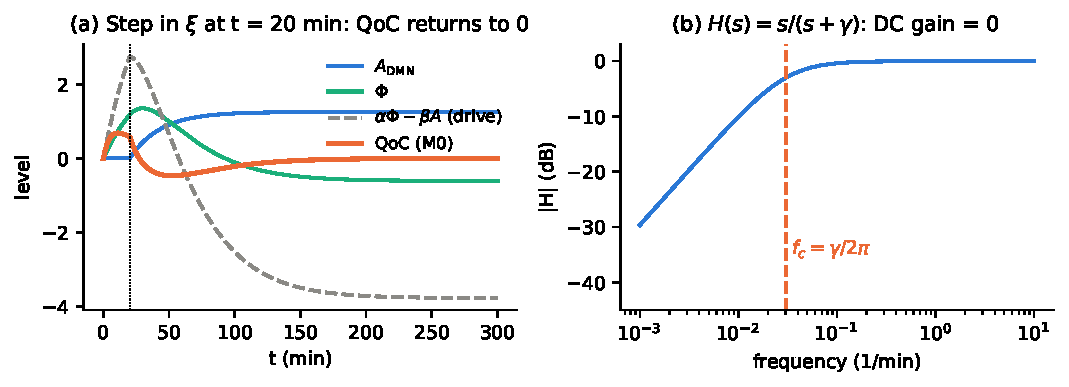
\includegraphics[width=\linewidth]{fig1_highpass_qoc.pdf}
\caption{Proposition~\ref{prop:p2} on the actual ODE \eqref{eq:m0A}--\eqref{eq:m0Q} with the printed parameters. (a)~A step in the drive $\xi$ at $t=20$~min moves $A$ and $\Phi$ to new levels and the drive $\alpha\Phi-\beta A$ to $-3.77$; QoC responds transiently and returns to zero (final value $-8\times10^{-9}$, attenuation $>10^{8}$). (b)~Bode magnitude of $H(s)=s/(s+\gamma)$: zero gain at DC, corner frequency $\gamma/2\pi$. Sinusoidal drives at $\omega=0.05,0.2,1.0$~rad/min reproduce $|H(j\omega)|$ with relative errors $0.14\,\%$, $0$, $0$.}
\label{fig:highpass}
\end{figure}

\Cref{tab:steady} and \Cref{fig:highpass} summarise Propositions~\ref{prop:p1}--\ref{prop:p3}. The equilibrium of M0 under zero-mean noise has $\QoC^*=0$ exactly, and the step response in \Cref{fig:highpass}a shows that this is not an artefact of the particular equilibrium: a sustained change of DMN activity and integration produces a sustained change of the \emph{drive} but no sustained QoC. The printed closed forms differ from the true equilibrium in all three components and their residual in the model equations is of order $\gamma\QoC^*_{\mathrm p}\approx5.3$ per minute, two orders of magnitude larger than the largest rate in the model.

\begin{figure}[t]
\centering
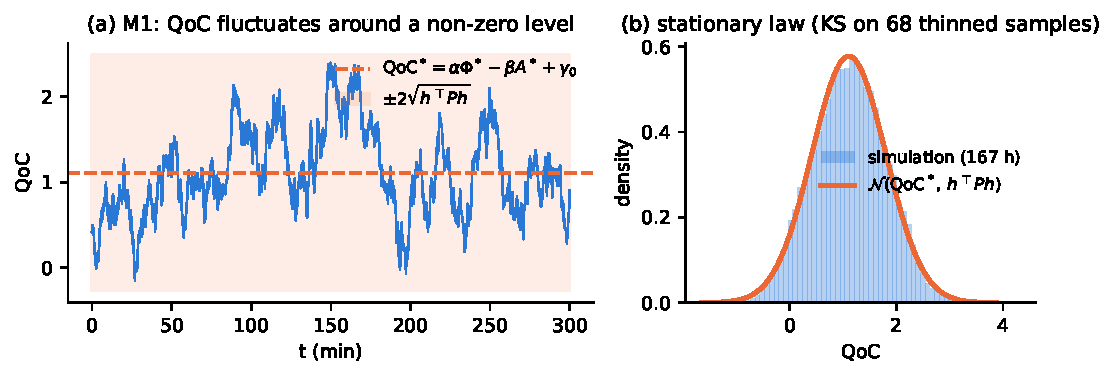
\includegraphics[width=\linewidth]{fig2_m1_stationary.pdf}
\caption{Propositions~\ref{prop:p4}--\ref{prop:p5} for M1 at the nominal parameters. (a)~A 300-min excerpt of a simulated session (exact discretisation, $\Delta=10$~s) fluctuating around $\QoC^*=1.108$; the band is $\pm2\sqrt{\hv^\top P\hv}$. (b)~Histogram of QoC over a $10^4$-min simulation against the closed-form $\mathcal N(\QoC^*,\hv^\top P\hv)$ (the panel title counts the thinned samples of this single run). The verification gate uses a Kolmogorov--Smirnov test on 2{,}000 thinned samples (one every five slowest time constants) pooled over five independent chains: $D=0.020$, $p=0.42$; errors of the sample mean and standard deviation $0.005$ and $0.007$.}
\label{fig:stationary}
\end{figure}

M1 removes the defect (\Cref{fig:stationary}). The Lyapunov residual of \eqref{eq:P} is zero to machine precision, the stationary level is $\QoC^*=1.108$ with variance $0.477$, and the empirical stationary law of a long simulation is indistinguishable from the predicted Gaussian. Pooling several independent chains for the Kolmogorov--Smirnov test is deliberate: a single path of an autocorrelated process can sit two to three standard errors from its mean for hundreds of thinned samples (one of twelve seeds examined gave $z=3.5$ on its own; the standard deviation of $z$ over seeds was $0.99$, i.e.\ no bias), and a verification gate must not depend on the luck of one seed.

\subsection{Identifiability}
\label{sec:res-ident}

\paragraph{Structural.} \Cref{tab:structural} gives the rank of the exact information matrix in the four observation configurations. With ratings only, six of the ten parameters that enter the likelihood are identifiable; four directions are null and the practical remedy is to fix $A_0$, $\alpha$, $\sA$ and $\kint$, i.e.\ to give up the scale of both latent variables and the baseline. Adding one EEG channel leaves exactly one null direction, and in both cases it is an exact symmetry of the model (\Cref{app:symmetry}): when $\Phi$ is not observed, $(\kint,\sPhi,\alpha)\mapsto(c\,\kint,c\,\sPhi,\alpha/c)$ leaves the law of all observations unchanged (the scale of $\Phi$ is arbitrary); when $A$ is not observed, the affine map $A\mapsto cA+(1-c)\Amax$ with $(\kint,A_0,\sA,\beta,\gamma_0)\mapsto(\kint/c,\;cA_0+(1-c)\Amax,\;c\sA,\;\beta/c,\;\gamma_0+\beta(1-c)/c)$ does the same (the scale of $A$ is anchored only by $\Amax$). The numerically computed null vectors coincide with the gradients of these one-parameter families. Only configuration (d), ratings plus both EEG channels, identifies all 12 parameters, with a well-conditioned information matrix (condition number 188 after normalisation).

\begin{table}[t]
\centering\small
\caption{Structural identifiability by Rothenberg's rank criterion (90-min session, probes every minute, $\gamma_0=0.3$). ``Absent'': the parameter does not enter the likelihood. The null directions of (b) and (c) are the exact symmetries of \Cref{app:symmetry}. The last column names the parameters that must be fixed to restore local identifiability.}
\label{tab:structural}
\footnotesize\setlength{\tabcolsep}{4pt}
\begin{tabular}{llcll}
\toprule
Configuration & Absent & Rank & Null direction(s) & Fix \\
\midrule
(a) ratings                      & $\rA,\rPhi$ & 6/10  & four (symmetries below $+$ noise scales) & $A_0,\alpha,\sA,\kint$ \\
(b) ratings $+\,y_A$             & $\rPhi$     & 10/11 & $\Phi$-scaling: $\kint,\sPhi\uparrow$, $\alpha\downarrow$ & $\alpha$ \\
(c) ratings $+\,y_\Phi$          & $\rA$       & 10/11 & $A$-affine: $\gamma_0,\beta,A_0,\kint\uparrow$, $\sA\downarrow$ & $\gamma_0$ \\
(d) ratings $+\,y_A+y_\Phi$      & --          & 12/12 & none & none \\
\bottomrule
\end{tabular}
\end{table}

\paragraph{Practical.} \Cref{tab:crb} lists the relative CRB at the reference design. Two patterns matter for design. First, the three rate constants $\kinh,\kint,\kd$ are the hardest parameters in every configuration (15--18\,\% in configuration (d), against 3\,\% for $A_0$ and 4--7\,\% for the gains). Second, the EEG channels do most of the work: ratings alone give $\CRB(\kinh)=556\,\%$ and $\CRB(\beta)=277\,\%$, i.e.\ no usable information, and a single channel already brings $\kinh$ to 16--48\,\% depending on which channel it is. The DMN channel is the one that matters for $\kinh$ and $A_0$ (configuration (b) is almost as good as (d) for them), the $\Phi$ channel for $\sPhi$ and $\alpha$.

\begin{table}[t]
\centering\small
\caption{Relative Cram\'er--Rao bound by observation configuration at the reference design ($N=12$, 45 min, probe every 2 min, $\rA=\rPhi=0.1$, $\rQ=0.3$). ``fixed'': normalisation of a non-identifiable direction (\Cref{tab:structural}); ``absent'': parameter does not enter the likelihood; for $\gamma_0=0$ the absolute standard error is given.}
\label{tab:crb}
\begin{tabular}{lcccc}
\toprule
 & (a) ratings & (b) ratings $+\,y_A$ & (c) ratings $+\,y_\Phi$ & (d) ratings $+\,y_A+y_\Phi$ \\
\midrule
$\kinh$   & 5.559 & 0.157 & 0.480 & 0.155 \\
$A_0$     & 0.325 & 0.031 & 0.170 & 0.030 \\
$\sA$     & fixed & 0.049 & 0.309 & 0.049 \\
$\kint$   & fixed & 0.260 & 0.254 & 0.175 \\
$\kd$     & 1.155 & 0.337 & 0.372 & 0.178 \\
$\sPhi$   & 8.607 & 0.175 & 0.063 & 0.057 \\
$\alpha$  & fixed & fixed & 0.092 & 0.037 \\
$\beta$   & 2.765 & 0.116 & 0.137 & 0.072 \\
$\gamma_0$& fixed & SE $=0.736$ & fixed & SE $=0.130$ \\
$\rA$     & absent & 0.016 & absent & 0.016 \\
$\rPhi$   & absent & absent & 0.014 & 0.014 \\
$\rQ$     & 0.212 & 0.070 & 0.122 & 0.050 \\
\bottomrule
\end{tabular}
\end{table}

\begin{figure}[t]
\centering
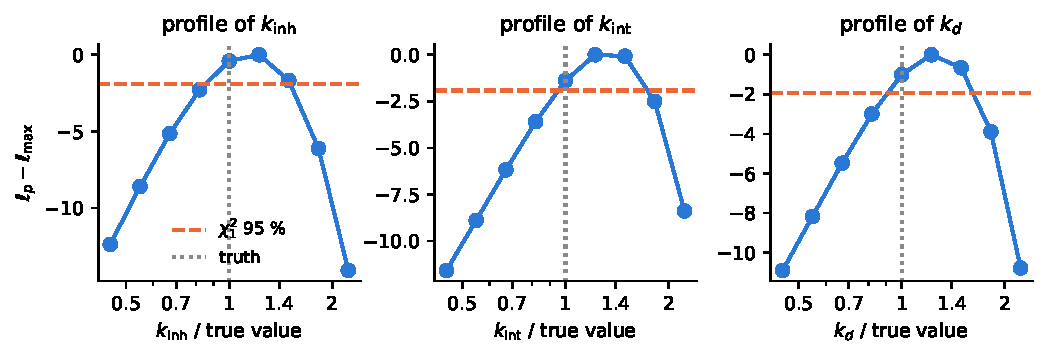
\includegraphics[width=\linewidth]{fig3_profiles.pdf}
\caption{Profile log-likelihoods of the three rate constants on one simulated data set of the reference design (configuration (d)), all other parameters re-optimised at each grid point. Dashed line: $\chi^2_1$ 95\,\% threshold ($-1.92$); dotted line: true value. Each profile is unimodal with its maximum within one grid step of the truth ($\kinh$: 0.244 vs 0.200; $\kint$: 0.099 vs 0.081; $\kd$: 0.042 vs 0.034), and the curvature implied by the drop of 8--14 log-likelihood units at $\pm0.8$ log units corresponds to relative standard errors of $0.15$--$0.20$, in line with the bounds of $0.16$--$0.18$ in \Cref{tab:crb}.}
\label{fig:profiles}
\end{figure}

The profile likelihoods in \Cref{fig:profiles} confirm that the rate constants are practically identifiable in configuration (d): no profile is flat or multimodal in the $\pm0.8$ log-unit window, and the likelihood-based 95\,\% intervals have widths consistent with the Fisher bounds.

\subsection{The bound predicts the error of maximum likelihood}
\label{sec:res-crbvalid}

\begin{figure}[t]
\centering
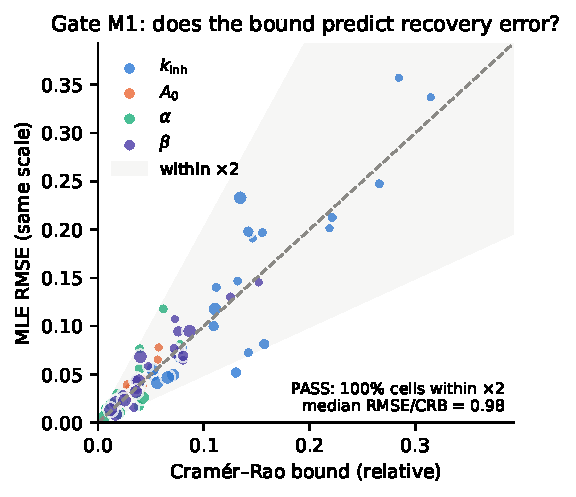
\includegraphics[width=0.55\linewidth]{fig4_crb_vs_mle.pdf}
\caption{Gate M1. Root-mean-square error of maximum-likelihood recovery (five independent data sets per cell, 24 design cells spanning the grid) against the relative Cram\'er--Rao bound, both in the same scale; marker size grows with $N$. The shaded region is a factor of two around the identity. All 24 cells pass; the median ratio $\RMSE/\CRB$ is $0.98$ (10th--90th percentiles $0.61$--$1.40$, extremes $0.40$ and $1.93$).}
\label{fig:crbvalid}
\end{figure}

\Cref{fig:crbvalid} compares the realised RMSE of the ML estimator with the CRB in 24 cells covering $N$ from 6 to 48, sessions from 20 to 90 minutes, all probe intervals and all noise levels. The ratio $\RMSE/\CRB$ has median $0.98$ and per-parameter medians $0.96$ ($\kinh$), $0.97$ ($A_0$), $1.00$ ($\alpha$) and $1.06$ ($\beta$); no ratio exceeds $2$ and the five ratios below $0.5$ (minimum $0.40$) are the sampling noise of an RMSE computed from five fits falling \emph{below} the bound, not evidence of a problem. The concern that the bound is optimistic at small $N$ does not materialise: in the four $N=6$ cells the ratios lie between $0.7$ and $1.5$. At the reference cell the bound predicts $(15.5,\,3.0,\,3.7,\,7.2)\,\%$ for $(\kinh,A_0,\alpha,\beta)$ and ML achieves $(19.7,\,2.6,\,3.8,\,7.7)\,\%$. We therefore use the exact CRB, which costs about two seconds per design, in place of simulation for the full design map.

\subsection{Design map}
\label{sec:res-design}

\begin{figure}[t]
\centering
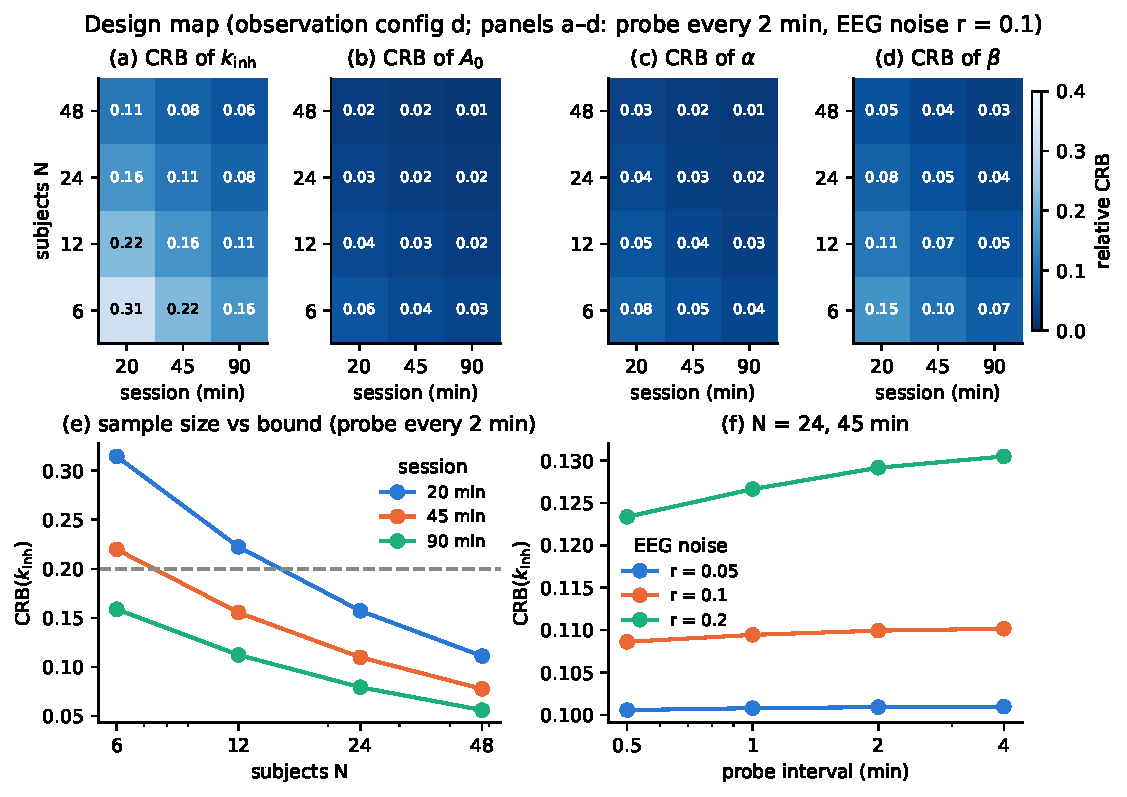
\includegraphics[width=\linewidth]{fig5_design_map.pdf}
\caption{Design map (configuration (d)). (a--d)~Relative CRB of $\kinh$, $A_0$, $\alpha$, $\beta$ as a function of the number of subjects and the session length, for probes every 2 min and EEG noise $r=0.1$; cells with values below 0.2 are adequate. (e)~$\CRB(\kinh)$ versus $N$ for the three session lengths; the dashed line is the 20\,\% criterion. (f)~Effect of the probe interval and of the EEG noise level on $\CRB(\kinh)$ at $N=24$, 45 min: the probe interval is irrelevant for $\kinh$, the EEG noise is not.}
\label{fig:designmap}
\end{figure}

\begin{table}[t]
\centering\small
\caption{Cheapest design in the grid (smallest $N\times T$, ties broken by the bound) with relative CRB $\le 20\,\%$ for each key parameter, and the fraction of the 144 grid cells that are adequate for it.}
\label{tab:mindesign}
\begin{tabular}{lrrrrrr}
\toprule
Parameter & $N$ & session (min) & probe (min) & EEG noise $r$ & CRB & adequate cells \\
\midrule
$\kinh$  & 24 & 20 & 0.5 & 0.05 & 0.142 & 75\,\% \\
$A_0$    & 6  & 20 & 0.5 & 0.05 & 0.057 & 100\,\% \\
$\alpha$ & 6  & 20 & 0.5 & 0.05 & 0.037 & 100\,\% \\
$\beta$  & 6  & 20 & 0.5 & 0.05 & 0.072 & 98\,\% \\
\bottomrule
\end{tabular}
\end{table}

\Cref{fig:designmap} and \Cref{tab:mindesign} are the central practical result. Three facts stand out.

\emph{The DMN inhibition rate is the bottleneck.} $A_0$ and $\alpha$ are adequately estimated in every one of the 144 designs, $\beta$ in all but the three smallest (6 subjects, 20 min, probes every 4 min), whereas $\kinh$ is adequate in 75\,\% of them and fails in every 6-subject design shorter than 90 minutes (worst case $38\,\%$ at $N=6$, 20 min, $r=0.2$). With probes every 2 minutes and 45-minute sessions, $N=12$ reaches $14.3$--$15.5\,\%$ for $\kinh$ at $r\le0.1$ and $18.3\,\%$ at $r=0.2$, while $N=6$ gives $22\,\%$.

\emph{Simple scaling rules.} A log-linear regression of the bound on the design variables over the 144 cells (\Cref{tab:scaling}) shows that every bound scales exactly as $N^{-1/2}$, as it must for independent subjects, and almost as $T^{-1/2}$ in the session length; the exponent of $T$ is slightly weaker for $\kinh$ ($-0.46$) and $A_0$ ($-0.39$) because each new subject contributes an independent draw from the stationary law whereas extra minutes of the same subject are autocorrelated. Many short sessions are therefore marginally better than few long ones for the DMN parameters and equivalent for the gains: at equal $NT$, 24 $\times$ 20 min gives $\CRB(A_0)=2.9\,\%$ against $3.2\,\%$ for 6 $\times$ 90 min. The remaining design variables act differently on different parameters: the probe interval has no effect on $\kinh$ and $A_0$ (which are informed by the dense EEG channel) but enters the gains $\alpha,\beta$ with exponent $\approx0.45$, i.e.\ halving the probe interval reduces their bound by about 27\,\%; the EEG noise affects $\kinh$ and the gains with exponent $\approx0.17$--$0.20$ and $A_0$ not at all. For $\kinh$ the rule reduces, to a good approximation, to a total-recording-time requirement: at $r\le0.1$ about $480$--$540$ subject-minutes of two-channel EEG (24 $\times$ 20 min, 12 $\times$ 45 min or 6 $\times$ 90 min) bring the bound to 15--16\,\%.

\begin{table}[t]
\centering\small
\caption{Exponents of the power-law fit $\CRB\propto N^{a}\,T^{b}\,r^{c}\,T_p^{d}$ over the 144 grid cells (log-linear least squares; $N$ subjects, $T$ session length, $r$ the EEG noise sd, $T_p$ the probe interval).}
\label{tab:scaling}
\begin{tabular}{lrrrr}
\toprule
Parameter & $a$ (subjects) & $b$ (session length) & $c$ (EEG noise) & $d$ (probe interval) \\
\midrule
$\kinh$  & $-0.50$ & $-0.46$ & $0.17$ & $0.01$ \\
$A_0$    & $-0.50$ & $-0.39$ & $0.02$ & $0.00$ \\
$\alpha$ & $-0.50$ & $-0.50$ & $0.17$ & $0.44$ \\
$\beta$  & $-0.50$ & $-0.50$ & $0.20$ & $0.45$ \\
\bottomrule
\end{tabular}
\end{table}

\emph{Probe schedules.} With 22 probes in a 45-minute session, the uniform schedule attained the smallest Ds-criterion among all schedules tested. The nearest competitors, mild front- or back-loading ($p=0.85$ and $1.15$), were within $0.05\,\%$ of it in geometric-mean standard error; strong front-loading ($p=0.4$) cost $1.2\,\%$, and paired probes one epoch apart cost $4.6\,\%$ (pairs 12 epochs apart $0.4\,\%$). Strong back-loading ($p\ge2.2$) collapses probes onto the same epochs and is infeasible. We make no claim of global optimality over all schedules; the result is that the common uniform schedule is not beaten by the usual non-uniform alternatives, because in configuration (d) the fast dynamics are already resolved by the EEG channels and the ratings mainly inform the static gains, for which spreading the probes evenly is natural.

\subsection{Closed-loop control}
\label{sec:res-control}

\begin{figure}[t]
\centering
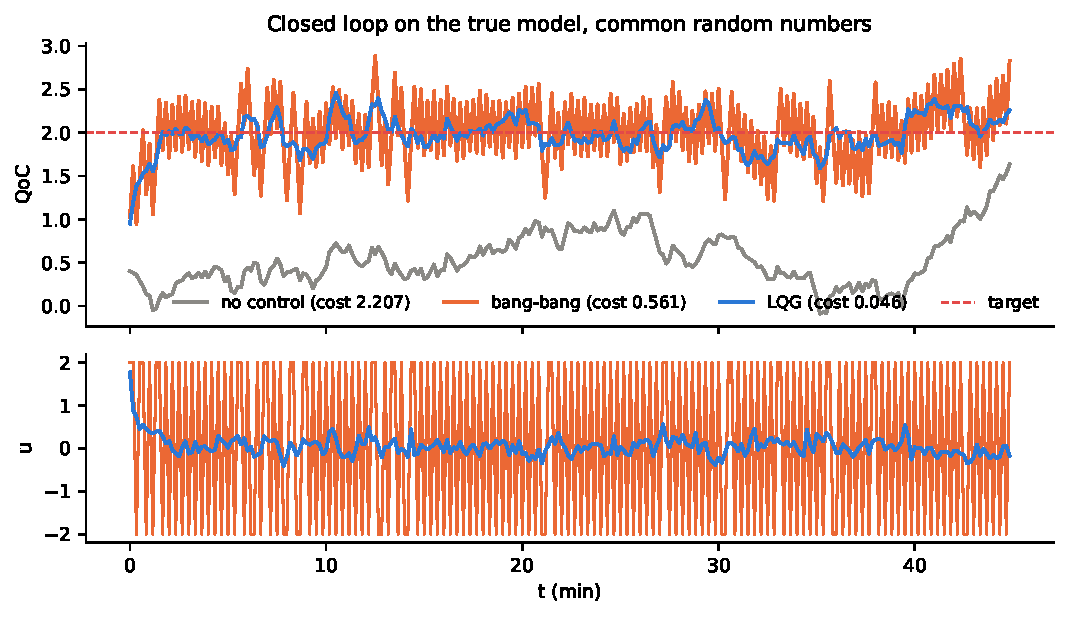
\includegraphics[width=\linewidth]{fig6_control_trajectories.pdf}
\caption{One 45-minute closed-loop session on the true model with common random numbers for the three policies (target $\QoC_{\mathrm{tgt}}=2.0$, $|u|\le2$). Top: QoC; bottom: input $u$. LQG holds QoC at the target with a small, smooth input; bang-bang chatters between $\pm u_{\max}$ and overshoots; without control QoC fluctuates around $\QoC^*=1.1$.}
\label{fig:control}
\end{figure}

\begin{table}[t]
\centering\small
\caption{Policy comparison on the true model (270 epochs, 20 trials, common random numbers). Cost $=\overline{(\QoC-\QoC_{\mathrm{tgt}})^2}+0.1\,\overline{u^2}$. The last row is the closed-form stationary value of the unclipped LQG loop (\Cref{app:lqg}); the corresponding long simulation gives $0.0346$ (difference 3\,\%).}
\label{tab:policies}
\begin{tabular}{lrrr}
\toprule
Policy & Cost & Tracking MSE & RMS input \\
\midrule
LQG (true parameters) & 0.039 & 0.035 & 0.22 \\
Bang-bang (same estimator) & 0.561 & 0.162 & 2.00 \\
No control & 1.481 & 1.481 & 0 \\
\midrule
LQG, stationary closed form & 0.034 & 0.030 & 0.18 \\
\bottomrule
\end{tabular}
\end{table}

\Cref{fig:control} and \Cref{tab:policies} summarise gate M2. With the true parameters, LQG achieves a session cost 14 times lower than bang-bang and 38 times lower than no control. The two neutral metrics tell the same story: LQG tracks the target with a mean-squared error of $0.035$ (about 7\,\% of the open-loop variance) while using an input of RMS $0.22$, whereas bang-bang tracks with an error of $0.16$ at the price of saturating the actuator all the time. The required mean input is small ($u_{\mathrm{ss}}=0.024$) because the target is only $0.9$ units above the open-loop level; the cost of LQG is dominated by the irreducible effect of process noise within one epoch, which is why its closed-form stationary cost ($0.034$) is close to the finite-horizon value. The comparison is made on the quadratic cost that LQG minimises; the point is not that bang-bang is a poor solution of \emph{its} problem, but that a model-based regulator exploiting the estimated state and the known dynamics is far more efficient at holding a level, which is the natural objective of a neurofeedback loop.

\begin{figure}[t]
\centering
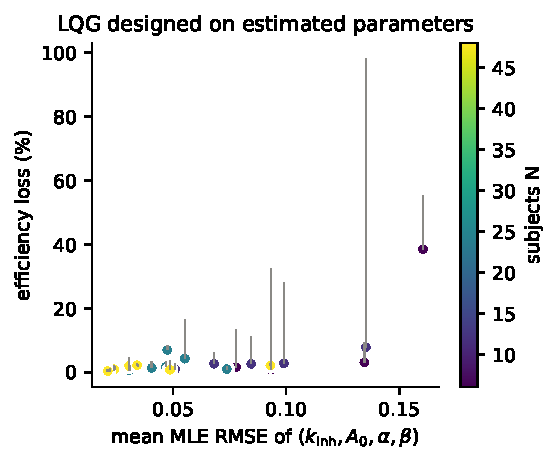
\includegraphics[width=0.6\linewidth]{fig7_robustness.pdf}
\caption{Robustness of LQG to parameter estimation error. For each of the 24 design cells, a controller (gain and filter) is designed on each of the five ML parameter sets recovered in that cell and run on the true model of that cell. Points: median efficiency loss over fits; whiskers extend to the 90th percentile; colour: number of subjects; horizontal axis: mean relative RMSE of $(\kinh,A_0,\alpha,\beta)$ in that cell. Full values in \Cref{tab:robust}.}
\label{fig:robustness}
\end{figure}

\Cref{fig:robustness} connects the design map to control. When the controller is designed on parameters estimated from a design that is adequate for $\kinh$ (19 of the 24 cells), the median loss of efficiency is a few per cent: $2.6\,\%$ (90th percentile $11\,\%$) at the reference design, $1.8\,\%$ ($3.4\,\%$) for 24 subjects $\times$ 45 min, below $1\,\%$ (90th percentile $\le 2.1\,\%$) for every 48-subject design at $r=0.05$, and at most $7\,\%$ (90th percentile at most $17\,\%$) over all adequate cells. The large losses all come from the five inadequate cells: 6 subjects $\times$ 20 min with probes every 2 min loses $38\,\%$ in the median and $55\,\%$ at the 90th percentile, and 12 subjects $\times$ 20 min at $r=0.2$ has a median loss of $8\,\%$ but a 90th percentile of $98\,\%$---one in ten controllers designed from such data would double the cost (two further inadequate cells have moderate medians but 90th percentiles of $28$--$32\,\%$). A design that cannot estimate the model therefore cannot support a model-based neurofeedback loop built on it, and the 20\,\% criterion of \Cref{sec:res-design} is, to a good approximation, the boundary between controllers that lose a few per cent and controllers that may lose most of their benefit.

\subsection{Global sensitivity}
\label{sec:res-sens}

\begin{figure}[t]
\centering
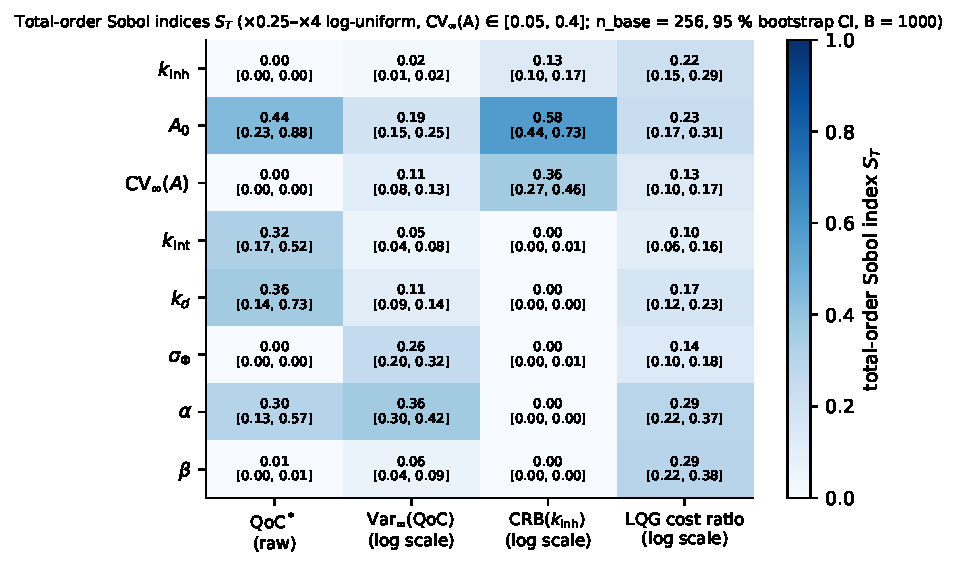
\includegraphics[width=0.8\linewidth]{fig8_sobol.pdf}
\caption{Total-order Sobol indices $S_T$ (with 95\,\% bootstrap intervals) of four outputs with respect to eight model parameters varied log-uniformly over $\times0.25$--$\times4$ around the nominal point ($\mathrm{CV}_A\in[0.05,0.4]$). $\Var_\infty(\QoC)$, $\CRB(\kinh)$ and the LQG efficiency are analysed on the log scale; $\QoC^*$ on the raw scale. Scrambled Sobol sampling, $n=256$, $2{,}560$ evaluations.}
\label{fig:sobol}
\end{figure}

\begin{table}[t]
\centering\small
\caption{Total-order Sobol indices $S_T$ with 95\,\% bootstrap confidence intervals ($B=1{,}000$). The last row is the convergence diagnostic $\max_i|\Delta S_{T,i}|$ between the full sample and its first half.}
\label{tab:sobol}
\footnotesize\setlength{\tabcolsep}{4pt}
\begin{tabular}{lcccc}
\toprule
Input & $\QoC^*$ (raw) & $\log\Var_\infty(\QoC)$ & $\log\CRB(\kinh)$ & $\log$ LQG efficiency \\
\midrule
$\kinh$          & 0.00 & 0.02 [0.01, 0.02] & 0.13 [0.10, 0.17] & 0.22 [0.15, 0.29] \\
$A_0$            & 0.44 [0.23, 0.88] & 0.19 [0.15, 0.25] & \textbf{0.58} [0.44, 0.73] & 0.23 [0.17, 0.31] \\
$\mathrm{CV}_A$  & 0.00 & 0.11 [0.08, 0.13] & \textbf{0.36} [0.27, 0.46] & 0.13 [0.10, 0.17] \\
$\kint$          & 0.32 [0.17, 0.52] & 0.05 [0.04, 0.08] & 0.00 & 0.10 [0.06, 0.16] \\
$\kd$            & 0.36 [0.14, 0.73] & 0.11 [0.09, 0.14] & 0.00 & 0.17 [0.12, 0.23] \\
$\sPhi$          & 0.00 & 0.26 [0.20, 0.32] & 0.00 & 0.14 [0.10, 0.18] \\
$\alpha$         & 0.30 [0.13, 0.57] & \textbf{0.36} [0.30, 0.42] & 0.00 & 0.29 [0.22, 0.37] \\
$\beta$          & 0.01 [0.00, 0.01] & 0.06 [0.04, 0.09] & 0.00 & 0.29 [0.22, 0.38] \\
\midrule
$\max|\Delta S_T|$ (half sample) & 0.10 & 0.013 & 0.076 & 0.030 \\
\bottomrule
\end{tabular}
\end{table}

\Cref{fig:sobol} and \Cref{tab:sobol} show which parameters the conclusions depend on.

\emph{Identifiability of $\kinh$ is set by the DMN baseline and its variability, not by $\kinh$.} The total index of $A_0$ on $\log\CRB(\kinh)$ is $0.58$ and that of $\mathrm{CV}_A$ is $0.36$, while $\kinh$ itself contributes $0.13$ and the remaining five parameters nothing. The first-order indices ($0.46$ and $0.25$) are smaller than the total ones, reflecting the interaction $A_0\times\mathrm{CV}_A$: what the EEG channel resolves is the amplitude of the DMN fluctuations, $\mathrm{CV}_A\cdot A_0$, relative to the observation noise. For an experimenter this means that the sample-size requirement for $\kinh$ depends on the signal-to-noise ratio of the DMN feature far more than on the (unknown) value of the rate itself, and that improving the DMN feature is worth more than adding probes.

\emph{Stationary variability is governed by the gain $\alpha$ and the $\Phi$ noise.} $\log\Var_\infty(\QoC)$ has $S_T=0.36$ for $\alpha$, $0.26$ for $\sPhi$ and $0.19$ for $A_0$; the indices are close to additive ($S_1\approx S_T$) and converged ($\max|\Delta S_T|=0.013$).

\emph{Control efficiency has no dominant parameter.} The LQG cost ratio spreads its sensitivity over $\beta,\alpha,A_0,\kinh,\kd$ ($S_T$ from $0.17$ to $0.29$) with small first-order indices, i.e.\ the benefit of closed-loop control is a joint property of the gains and the DMN dynamics; no single parameter can make or break it within the range explored.

\emph{The stationary level $\QoC^*$} depends on $A_0,\kd,\kint,\alpha$ and not on $\beta$ (because $\QoC^*=\alpha\kint(1-A_0)/\kd-\beta A_0$ and the first term dominates). Its indices sum to more than one and have wide intervals (convergence $0.10$) because the output is a product of inputs on the raw scale; we only retain the ordering.

\subsection{Application to an experience-sampling EEG dataset}
\label{sec:res-real}

The design analysis makes two predictions that can be checked on data: how precisely the rate constants can be estimated from a real experience-sampling design, and whether a model that is identifiable in principle predicts the reported state better than simpler models. We tested both on ds001787 \citep{Delorme2024ds,Brandmeyer2018}, the open dataset on which the reference design of \Cref{sec:grid} was patterned. The analysis followed a preregistration that was locked with a SHA-256 hash after the rating decoding and the structural analysis on the real probe schedules, and before any EEG sample was downloaded (lock at 13:48 UTC on 19 October 2026, first EEG file at 13:49 UTC). Metadata and behavioural files were inspected before locking; the EEG was not. Every locked analysis is reported, including those that did not support the predictions, and all deviations are listed in \Cref{app:realdata}.

\paragraph{Data, features and model.} The dataset contains 40 sessions (16--60~min, median 45~min) from 24 practitioners of Himalayan Yoga mantra meditation, 12 experienced and 12 novices, with 64-channel EEG at 256~Hz and 983 experience-sampling probes. Each probe asks three questions on a 0--3 scale: depth of meditation (Q1), depth of mind wandering (Q2) and drowsiness (Q3). The rating is $r=\mathrm{Q1}-\mathrm{Q2}$, from $-3$ to $3$. Key presses were decoded from the behavioural logs because a key of 0 leaves no trigger in the event files (gate E0: 96.6\,\% of probes matched; none of 741 zero-key presses has a trigger). The EEG was band-passed at 1--40~Hz with a 50~Hz notch, bad channels were interpolated and the data re-referenced to the average. Eye and muscle components identified by ICLabel \citep{PionTonachini2019} with probability at least 0.8 were removed from an extended-infomax Picard decomposition \citep{Ablin2018} of a 1--100~Hz copy of the same data; preprocessing used MNE-Python \citep{Gramfort2013}. Each session was cut into a continuous grid of 10-s epochs. An epoch that overlapped a probe window or exceeded $150~\mu$V peak-to-peak on any channel was marked missing rather than deleted, so the time step of the model is preserved and the Kalman filter skips the update (\Cref{app:kalman}). The DMN proxy $y_A$ is the log 8--12~Hz power over nine posterior channels. The integration proxy $y_\Phi$ is the multichannel Lempel--Ziv complexity \citep{Schartner2015} of 19 channels, standardised against 20 phase-randomised surrogates to remove its spectral component. Both are centred within each session and divided by one pooled within-session standard deviation. Ratings are centred within session and enter the filter as observations at the exact probe times, with the exact discretisation of \Cref{sec:disc} applied to the irregular steps. After centring, the levels $A_0$, $\Phi^*$ and $\gamma_0$ are not estimable (the affine symmetry of \Cref{app:symmetry}), so M1 is fitted in deviation form, $\dd\tilde\xv=M\tilde\xv\,\dd t+G\,\dd\mathbf W$ with $M=\bigl(\begin{smallmatrix}-\kinh&0\\-\kappa&-\kd\end{smallmatrix}\bigr)$ and $\kappa=\kint/\Amax$. Its ten free parameters are $(\kinh,\kappa,\kd,\sA,\sPhi,\alpha,\beta,\rA,\rPhi,\rQ)$, with free signs for $\kappa$, $\alpha$ and $\beta$. The pooled maximum-likelihood fit used six starting points.

\paragraph{Gates and retained data.} The decoding gate (E0) and structural identifiability on the real probe schedules (E1: rank 10/10; predicted relative CRB of $\kinh$ 9.1\,\% for the 40 sessions at the nominal parameters) passed before the lock. The features showed temporal structure (median lag-1 autocorrelation of $y_A$ 0.42, above the stop threshold of 0.3). The locked artefact rule retained 22 of 40 sessions: 12 experienced and 10 novices from 16 subjects, with 554 rated probes and a median of 30\,\% missing epochs. The loss of 45\,\% is below the stop threshold of 50\,\% but is not random; it is driven by temporal muscle artefact and by sessions with globally high amplitude (\Cref{app:realdata}). Practical identifiability (E2) and the model checks (E3) passed, and the four gates were recorded in order. \Cref{fig:real-session} shows one retained session as the fitted model sees it.

\begin{figure}[tbp]
\centering
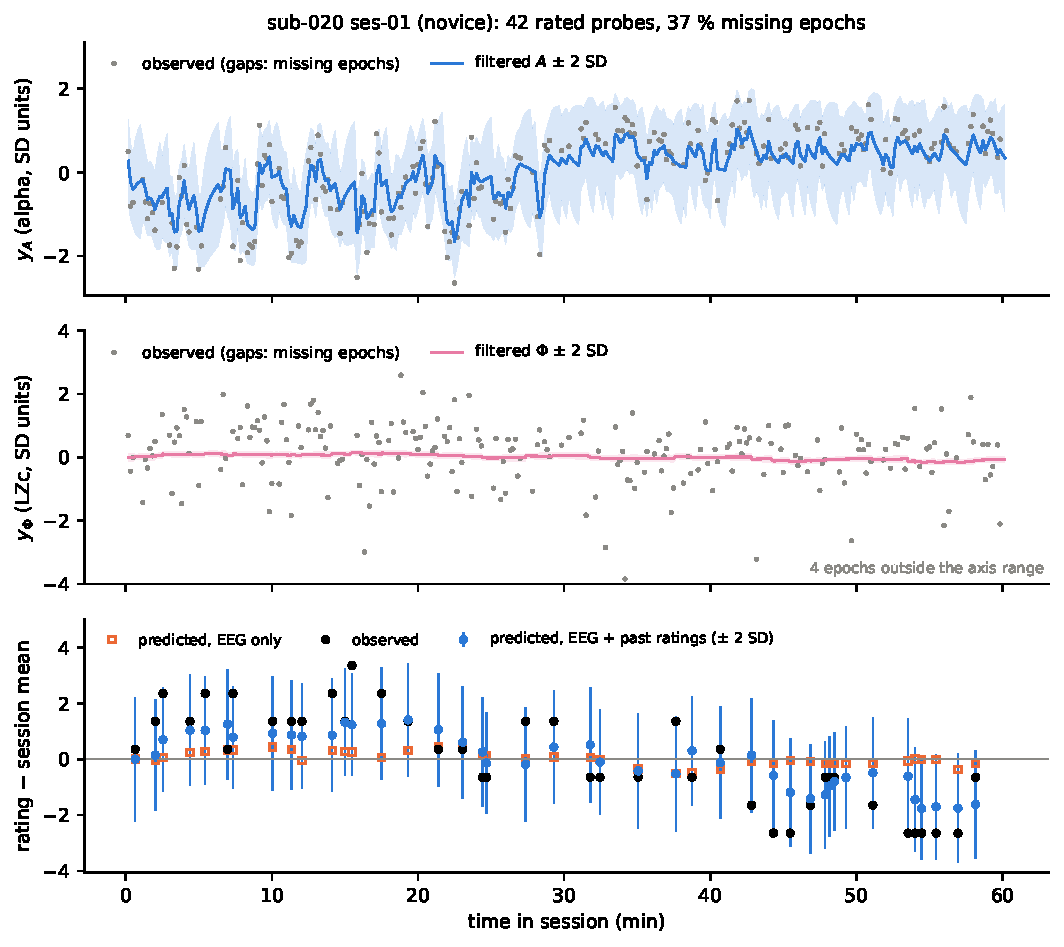
\includegraphics[width=0.9\linewidth]{fig9_realdata_session.pdf}
\caption{One session of ds001787 filtered with M1 at the pooled estimate (in sample): the retained session with the most rated probes, chosen by that rule (sub-020 ses-01, novice). Top: DMN proxy $y_A$ and the filtered $A\pm2$ SD. Middle: integration proxy $y_\Phi$ and the filtered $\Phi\pm2$ SD, which hardly moves because $y_\Phi$ is almost pure noise; four outlying epochs lie outside the axis. Bottom: ratings centred within session, with one-step-ahead predictions from EEG and past ratings ($\pm2$ SD) and from EEG alone. Gaps in the EEG series are missing epochs (probe windows and amplitude rule).}
\label{fig:real-session}
\end{figure}

\paragraph{Estimates and the three error numbers.} The DMN proxy relaxes fast: $\hat k_{\mathrm{inh}}=1.32~\mathrm{min^{-1}}$, a time constant of 0.76~min with 95\,\% profile interval 0.49--1.17~min, against the nominal 5~min and the 23~min printed with M0. The latent integration variable relaxes with $1/\hat k_d=5.0$~min (3.1--8.7~min). The coupling $\kappa$ is not distinguishable from zero (relative SE 151\,\%), and its profile is flat (\Cref{fig:real-profiles}). The two proxies differ sharply in quality. The DMN channel has a signal-to-noise ratio $\mathrm{sd}_\infty(A)/\rA=1.11$ against a nominal 1.58, whereas the integration channel has $0.06$ against a nominal 2.4: the spectrum-controlled LZc carries almost no slow signal.

\Cref{tab:real-errors} places the three preregistered error numbers side by side. The parametric bootstrap \citep{Efron1993} reproduces the Fisher standard error at the MLE, with ratios from 0.98 to 1.69; this is gate E2, the real-design counterpart of \Cref{fig:crbvalid}. In Fisher terms the design analysis was accurate. The bound for $\kinh$ computed before any EEG was seen (9.1\,\%) and the bound recomputed at the measured signal-to-noise ratio on the retained sessions (13.3\,\%) bracket the 9.9\,\% achieved; the achieved error is the smaller of the two recomputed values because the fitted rate is about six times the nominal one, so a session contains more independent DMN fluctuations. The observed information tells a different story for the DMN channel. The numerical Hessian gives 22.8\,\% for $\kinh$ and the profile likelihood 21.9\,\%, more than twice the Fisher value. The same factor, 2.1--2.5, appears for $\sA$ and $\rA$, whereas for $\kd$, $\rPhi$ and $\rQ$ observed and expected information agree within 5\,\%. In one data set simulated from $\hat\thetav$ on the same 22 designs the factor for $\kinh$, $\sA$ and $\rA$ is 1.05--1.07. A gap between observed and expected information that is confined to one channel and absent under the fitted model is the signature of misspecification of that channel \citep{White1982}: posterior alpha power is not fully described by one Ornstein--Uhlenbeck process plus white noise. (For $\alpha$ and $\sPhi$ the two informations differ in real and simulated data alike, a consequence of their near trade-off discussed below.) Because the bootstrap simulates from the model, it cannot detect the misspecification, and we report the profile interval as the uncertainty of $\kinh$. Hypothesis E-H1 is supported under its preregistered criterion, a Fisher SE of at most 20\,\% with $\RMSE/\mathrm{SE}\in[0.5,2]$, but not with the likelihood-based SE.

\begin{table}[t]
\centering\small
\caption{Three error numbers on ds001787 for the key parameters (rates in min$^{-1}$), as relative errors (standard error of the logarithm for the rates, $\mathrm{SE}/|\hat\theta|$ for the gains). Predicted CRB: exact Fisher information at the nominal parameters on the 40 real designs before the lock (E1), then on the 22 retained designs, then on these designs with $\rA$ set to the measured signal-to-noise ratio of the DMN channel. SE at the MLE: expected Fisher information at $\hat\thetav$, and the observed information from the numerical Hessian of the log-likelihood. RMSE: 200 parametric-bootstrap refits on the real designs. The rates are scale-free and the columns are comparable; for the gains the predicted CRB refers to the nominal values ($\alpha=2.34$, $\beta=1.87$) and is not comparable with the errors at the estimates. The relative error of $\beta$ is large because $\hat\beta\approx0$.}
\label{tab:real-errors}
\footnotesize\setlength{\tabcolsep}{3.5pt}
\begin{tabular}{lrrrrrrrr}
\toprule
 & & \multicolumn{3}{c}{Predicted CRB} & \multicolumn{2}{c}{SE at the MLE} & & \\
\cmidrule(lr){3-5}\cmidrule(lr){6-7}
 & Estimate & 40 designs & 22 designs & measured SNR & Fisher & observed & RMSE & RMSE/SE \\
\midrule
$\kinh$              & 1.32     & 0.091 & 0.123 & 0.133 & 0.099 & 0.228 & 0.097 & 0.98 \\
$\kd$                & 0.200    & 0.141 & 0.190 & 0.191 & 0.254 & 0.267 & 0.257 & 1.01 \\
$\alpha$             & 13.1     & 0.020 & 0.027 & 0.028 & 0.318 & 0.474 & 0.539 & 1.69 \\
$\beta$              & $-0.026$ & 0.040 & 0.054 & 0.057 & 3.14  & 3.79  & 3.15  & 1.00 \\
\bottomrule
\end{tabular}
\end{table}

\begin{figure}[tbp]
\centering
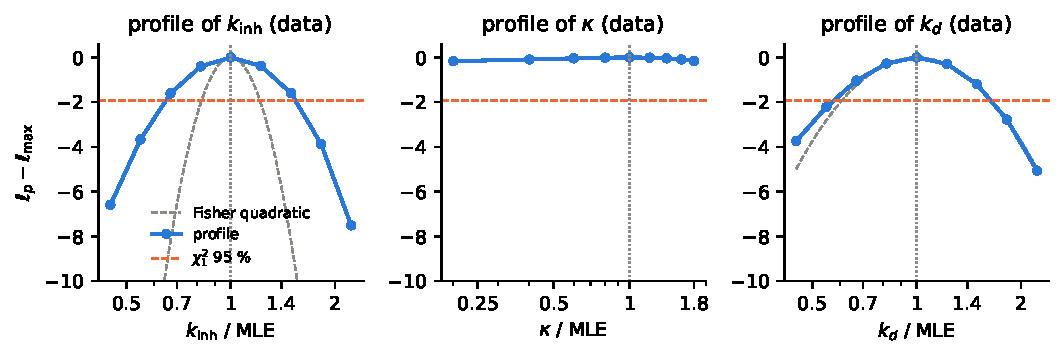
\includegraphics[width=\linewidth]{fig10_realdata_profiles.pdf}
\caption{Profile log-likelihoods of the three rate constants on ds001787, all other parameters re-optimised at each point (compare \Cref{fig:profiles}). Grey dashed: quadratic approximation implied by the expected Fisher information at the MLE; orange: $\chi^2_1$ 95\,\% threshold. The profile of $\kd$ follows the Fisher quadratic. That of $\kinh$ is about twice as wide (95\,\% interval 0.86--2.03~min$^{-1}$), the misspecification signature discussed in the text. The profile of $\kappa$ is flat over $\hat\kappa\times[0.2,1.8]$ because $\hat\kappa\approx0$.}
\label{fig:real-profiles}
\end{figure}

\paragraph{Gains.} The gain from the integration variable to the rating is positive, $\hat\alpha=13.1$ (Fisher 95\,\% CI 4.9--21.3; no bootstrap replicate at or below zero), as predicted by hypothesis E-H3. Its meaning is limited, however. Since $y_\Phi$ is essentially noise, the latent $\Phi$ is identified almost entirely by the ratings themselves. $\alpha$ and $\sPhi$ then trade off (bootstrap correlation of $\log\sPhi$ and $\alpha$: $-0.83$), which produces a long upper tail in the bootstrap distribution of $\alpha$ (2.5--97.5\,\% range 8.8--33.0) and its ratio of 1.69, and only the contribution of $\Phi$ to the rating variance is well determined. The result should not be read as a positive relation between LZc and the reports. The DMN gain is $\hat\beta=-0.03$ (95\,\% CI $-0.19$ to $0.14$): the sign asked for by E-H4 is not determined, and posterior alpha power makes no detectable contribution to the ratings.

\paragraph{Out-of-sample prediction.} \Cref{tab:real-loso} gives the leave-one-session-out comparison of hypothesis E-H2 on 554 probes. With EEG only, M1 predicts the ratings no better than an instantaneous regression on the two features (N2). With EEG and past ratings, M1 beats the running session mean (N3) but not M1 fitted to the ratings alone (N1), which has the best log predictive density and the smallest error of all models. The advantage over N3 therefore comes from the serial dependence of the reports, not from the EEG, and E-H2 is not supported. The session of \Cref{fig:real-session} shows the pattern: the filtered DMN proxy follows $y_A$, the filtered $\Phi$ barely moves, and the predictions from EEG alone stay near zero while those that use past ratings track the slow drift of the reports.

\begin{table}[t]
\centering\small
\caption{Leave-one-session-out prediction of the ratings (554 probes, 22 sessions; hypothesis E-H2), (a) from EEG only and (b) from EEG and past ratings. LPD: mean Gaussian log predictive density per probe; MAE: mean absolute error. $\Delta$LPD: M1 minus null model, averaged within session first, with a session-level bootstrap 95\,\% interval (2{,}000 resamples). N2: instantaneous regression of the rating on $(y_A,y_\Phi)$ at the probe epoch; N1: M1 with the rating channel only; N3: running mean of the session's past ratings.}
\label{tab:real-loso}
\footnotesize\setlength{\tabcolsep}{4pt}
\begin{tabular}{lrrrrr}
\toprule
Comparison & LPD M1 & LPD null & $\Delta$LPD [95\,\% CI] & MAE M1 & MAE null \\
\midrule
(a) M1 vs N2 & $-1.546$ & $-1.541$ & $-0.010$ [$-0.039$, $0.017$] & 0.93 & 0.92 \\
(b) M1 vs N1 & $-1.472$ & $-1.421$ & $-0.031$ [$-0.103$, $0.009$] & 0.88 & 0.84 \\
(b) M1 vs N3 & $-1.472$ & $-1.626$ & $+0.154$ [$0.083$, $0.233$] & 0.88 & 1.00 \\
\bottomrule
\end{tabular}
\end{table}

\paragraph{Groups and subjects.} Fitted separately, the experienced group has a smaller $\kinh$ than the novices (log difference $-1.19$, Wald 95\,\% CI $-1.56$ to $-0.81$), opposite to hypothesis E-H5. The two separate fits differ mainly in how the alpha-power variance is split between state and observation noise (signal-to-noise ratio 1.05 against 2.23), and $\kinh$ trades off against that split. When all other parameters are shared, the log difference shrinks to $-0.18$ and the preregistered one-degree-of-freedom likelihood-ratio test is not significant ($\chi^2_1=3.3$, $p=0.068$), although the groups differ in some parameter ($\chi^2_{10}=41.4$, $p<10^{-5}$, all parameters group-specific). E-H5 is not supported. The groups also differ in sex and age (10 of 12 against 2 of 12 men, mean age 39 against 48 years). Per-subject fits gave finite standard errors for 9 of 16 subjects; for the others the Fisher information was singular, in five cases because $\sPhi$ was estimated at zero. The random-effects meta-analysis \citep{Viechtbauer2005} of these nine gives a DMN time constant of 0.95~min (0.40--2.26~min) with large heterogeneity ($\tau=1.19$ log units, $I^2=0.92$).

\paragraph{Model checks and robustness.} The innovations are close to white, with median Ljung--Box \citep{Ljung1978} $p=0.27$ for $y_A$ and $0.40$ for $y_\Phi$ against the threshold of 0.01, although four of the 22 sessions have $p<0.01$ for $y_A$. The innovations of the two channels are uncorrelated (median $0.05$), so the diagonal observation noise of \eqref{eq:obsEEG} was kept. A posterior predictive check of the ordinal ratings (\Cref{tab:real-ppc}) reproduces their serial dependence (median lag-1 autocorrelation 0.22, simulated 0.26 with 95\,\% band 0.15--0.37) and the frequency of the extreme levels, but not the centre of the distribution: the data contain fewer ratings of 0 and more of $+1$ than a Gaussian read-out produces, and the experienced practitioners give less variable ratings than the pooled model implies. Across the six locked sensitivity analyses (\Cref{tab:real-sens}), $\alpha$ stays positive in all six. The sign of $\beta$ is kept in four, and the DMN time constant stays inside the main profile interval in four: the frontal-theta proxy gives 4.0~min, and the variant restricted to sessions with at most 20\,\% missing epochs keeps two sessions and gives a degenerate fit. The preregistered robustness rule, at least four of five analyses, is therefore met for $\alpha$ only, and we state the real-data results descriptively. A post-registration artefact rule that retains 39 sessions again gives a sub-minute DMN time constant (0.48~min), but a faster latent rating process ($1/\kd=1.7$~min) and $\hat\beta=+0.21$.

In short, on ds001787 (22 of 40 sessions, 554 rated probes) the DMN rate constant was estimated with a relative error of 10\,\% by the Fisher information, against 9--13\,\% predicted by the design analysis, but 22\,\% by the profile likelihood, and M1 did not predict ratings out of sample better than an instantaneous regression on the EEG features.

%% ─────────────────────────────────────────────────────────────────────────────
\section{Discussion}
\label{sec:discussion}

\paragraph{A consistency check that should precede fitting.} The first result is negative but, we think, instructive beyond the particular model: a differential equation in which the ``conscious'' variable is driven only by the time derivatives of its inputs cannot represent a sustained state, whatever its parameters. Substituting a proposed steady state back into the model equations (Proposition~\ref{prop:p3}) is a short calculation that we recommend as a routine step before any such model is fitted. The repaired model M1 keeps the mechanistic story of M0---practice suppresses the DMN, DMN disengagement feeds integration, both feed the reported quality---but turns it into a well-posed stationary stochastic process with closed-form moments. That it is linear-Gaussian is a modelling choice with a large pay-off: it makes the likelihood, the Fisher information and the optimal controller exact, which is what allows a complete design analysis without simulation.

\paragraph{What experience-sampling designs can and cannot deliver.} The identifiability analysis gives a clear hierarchy. Ratings alone are not enough to learn the dynamics: without an EEG channel the scales of both latent variables are arbitrary and the rate constants are known to within factors of several. One EEG channel removes all but one exact symmetry, and the symmetry is interpretable (the unobserved variable can be rescaled). Both channels identify everything. Within the identifiable configuration, the design map and the scaling rules of \Cref{tab:scaling} translate into advice an experimenter can use directly: (i) the number of probes governs the precision of the gains that link the latent state to the report, with a square-root-like return; (ii) the precision of the DMN rate constant depends on the total amount of EEG recorded and on the quality of the DMN feature, and not on how often one probes; (iii) about eight subject-hours of two-channel EEG at a feature noise of 10\,\% of the signal scale bring the rate constant to a 15\,\% relative error, and six-subject studies with sessions under 90 minutes cannot; (iv) uniform probe schedules are a safe default. These statements are about a model, not about brains, but they are exactly the kind of statement that must be available before a study is run if the study is meant to estimate a dynamical model, and they are absent from the current literature on computational models of meditation \citep{Laukkonen2021,SandvedSmith2021}, which has so far been descriptive.

\paragraph{From estimation to intervention.} The control analysis shows what a model buys once it is identified. A regulator that uses the state estimate and the known dynamics holds the reported quantity at a target with an input an order of magnitude smaller than a threshold policy and a tracking error more than four times smaller, and its performance can be predicted in closed form. More importantly, \Cref{fig:robustness} quantifies the cost of estimation error in the currency of the application: controllers designed from adequate designs lose a few per cent, controllers designed from inadequate designs may lose most of their benefit. This gives the 20\,\% identifiability criterion an operational meaning and argues for treating the design of the estimation study and the design of the neurofeedback protocol as one problem, in line with recent calls for more rigorous neurofeedback methodology \citep{Ros2020,Sitaram2017}.

\paragraph{Robustness of the conclusions.} The sensitivity analysis shows that the difficulty of estimating $\kinh$ is not a peculiarity of the nominal point: across a 16-fold range of every parameter it is controlled by the DMN baseline and coefficient of variation, both of which are properties of the EEG feature rather than of the rate. The conclusions about control efficiency and stationary variability are likewise spread over several parameters rather than hinging on one.

\paragraph{What the real data add.} The application to ds001787 (\Cref{sec:res-real}) supports the design analysis where it is a statement about information and qualifies it where it rests on the model being right. In Fisher terms the analysis was accurate: the bound computed before any EEG was seen and the bound at the measured signal-to-noise ratio bracket the error achieved, and the parametric bootstrap reproduced the bound on real, gap-ridden designs. What a design analysis cannot anticipate is misspecification. For the alpha-power proxy the observed information and the profile likelihood give errors more than twice the expected-information value, so design-map numbers should be read as lower bounds whenever a proxy is not known to follow the model, and likelihood-based intervals should be reported beside Fisher-based ones. The second lesson concerns the observation model rather than the dynamics. The two proxies we preregistered carried no detectable information about the reports beyond the reports' own serial dependence: the LZc channel was almost pure noise, posterior alpha did not load on the ratings, and out-of-sample prediction did not improve when EEG was added. Finding an EEG feature that tracks the reported state, with a signal-to-noise ratio in the range that \Cref{sec:res-design} shows to be necessary, is the open problem that the model leaves to experimenters.

\subsection{Limitations}
\label{sec:limitations}

\begin{itemize}
  \item \textbf{One dataset and uncalibrated proxies.} The design analysis is \emph{in silico}, and its only empirical test is one dataset (\Cref{sec:res-real}). There the preregistered artefact rule excluded 18 of 40 sessions non-randomly; the EEG features are proxies without a calibrated mapping to $A$ or $\Phi$ (posterior alpha is not a measure of DMN activity, LZc is not a measure of $\Phi$); the levels $A_0$, $\Phi^*$ and $\gamma_0$ are not estimable; the alpha channel shows signs of misspecification; and the group comparison is confounded by sex and age. The nominal point of the simulations is a working point; the sensitivity analysis covers a wide range around it but not qualitatively different regimes.
  \item \textbf{Linearity and Gaussianity.} M1 is linear with additive Gaussian noise and a linear read-out, and ratings are treated as continuous. Real ratings are ordinal and bounded, the DMN level is confined to $[0,\Amax]$, and meditation dynamics may involve discrete state switches \citep{Hasenkamp2012,Christoff2016}. On ds001787 the Gaussian read-out reproduced the serial dependence and the extreme levels of the ratings but not their skewed centre (\Cref{tab:real-ppc}). Non-linear extensions (saturating read-out, state-dependent noise, regime switching) would require approximate filters and simulation-based Fisher information; the present analysis is the exact baseline against which such extensions can be compared.
  \item \textbf{The mapping of EEG features to $(A,\Phi)$} is assumed, with noise levels as design variables. Establishing such a mapping is an empirical task; our results say how good it must be ($r\lesssim0.1$--$0.2$ of the signal scale) for the dynamics to be identifiable.
  \item \textbf{The design map is expressed in minutes at the nominal rates.} Session lengths of 20--90 min correspond to 4--18 DMN time constants at $\kinh=0.2$ but to only 0.9--3.9 at the printed value $0.043\ \mathrm{min^{-1}}$. The sensitivity analysis shows that $\CRB(\kinh)$ depends only weakly on $\kinh$ itself within $\times0.25$--$\times4$ ($S_T=0.13$), but a reader who expects much slower DMN dynamics should rescale session length in units of $1/\kinh$ and expect the requirement to shift towards longer sessions.
  \item \textbf{Probe burden is not costed.} Dense probing (every 30~s) improves the gains in the map but interrupts the practice it is meant to measure; the map should be read together with a ceiling on the number of probes that a protocol tolerates, which is outside the model.
  \item \textbf{Probe-schedule optimisation} was restricted to two interpretable families; a free optimisation over probe positions could find better schedules, although the small gaps we observe suggest limited room for improvement in configuration (d).
  \item \textbf{Control} assumes an additive input to the DMN equation with a known gain, perfect actuation within bounds and no delay, and compares policies on a quadratic cost. The robustness analysis covers parameter error but not model-structure error.
  \item \textbf{Between-subject heterogeneity} is not modelled: subjects share one parameter vector. A hierarchical extension would change the design map quantitatively (more subjects, shorter sessions) but not the identifiability structure. On ds001787 the between-subject standard deviation of $\log\kinh$ was 1.19 ($I^2=0.92$), so the pooled fit there describes an average practitioner at best.
\end{itemize}

\section{Conclusion}
\label{sec:conclusion}

For a recently proposed DMN--$\Phi$--QoC model of meditation dynamics we have shown that the original formulation has no sustained QoC, proposed a linear-Gaussian replacement with closed-form stationary behaviour, established exactly which observation configurations identify its parameters, validated the Cram\'er--Rao bound against maximum likelihood across the design space, derived a quantitative design map and scaling rules for the number of subjects, session length, probe interval and EEG quality, formulated and solved the closed-loop control problem, and quantified how estimation error from each design propagates to control performance. A preregistered application to open experience-sampling EEG data confirmed the Fisher-based predictions of the design analysis on a real design with gaps, exposed a misspecification of the alpha-power proxy that doubles the actual uncertainty of the DMN rate, and found no out-of-sample value of the two EEG proxies for predicting the reported state. The combination of exact Fisher information, machine-checked verification gates, preregistration and a single reproducible command is, we believe, a template for how dynamical models of mental states should be examined before and when they are taken to data.

%% ─────────────────────────────────────────────────────────────────────────────
\section*{Data and code availability}
The real-data application uses the open dataset ds001787 \citep{Delorme2024ds}, released under CC0 (\path{https://doi.org/10.18112/openneuro.ds001787.v1.1.1}) and described by Brandmeyer and Delorme \citep{Brandmeyer2018}. All other results are generated \emph{in silico}. Everything is produced by the accompanying Python code with seed 42: the model and design analysis by \path{bqi/dmn_ode.py}, \path{model/}, \path{eeg/model_fit.py} and \path{experiments/run_model_paper.py}, the real-data analysis by \path{eeg/realdata_features.py}, \path{model/realdata.py} and \path{experiments/run_realdata.py}. The preregistration and its SHA-256 lock are in \path{preregistration/}; the configuration snapshot, raw results, gate records and figures are in \path{outputs/}. The repository and a frozen archive with a DOI will be made public upon acceptance.

\section*{Acknowledgements}
This work was carried out at Phenikaa University, Hanoi. All computations were run on personal computers; no external funding was received. % TODO: add funding or grant number if applicable.

\section*{Author contributions}
D.V.\ conceived the study, developed the methodology and software, performed the analysis and wrote the manuscript.

\section*{Declaration of competing interest}
The author declares no competing interests. The author is also the author of the original model examined in this paper \citep{BQI}; the corrections in \Cref{sec:m0wrong} are reported here as part of the present analysis.

%% ─────────────────────────────────────────────────────────────────────────────
\appendix
\section{Proofs of Propositions~\ref{prop:p1}--\ref{prop:p5}}
\label{app:proofs}

\begin{proof}[Proof of Proposition~\ref{prop:p1}]
At an equilibrium with constant drive $\bar\xi$, \eqref{eq:m0A} gives $A^*=\kspont\bar\xi/\kinh$ and \eqref{eq:m0Phi} gives $\Phi^*=(\kint/\kd)(1-A^*/\Amax)$. With $\dot A=\dot\Phi=0$, \eqref{eq:m0Q} reduces to $0=-\gamma\QoC^*$, hence $\QoC^*=0$ since $\gamma>0$. The linear system is lower-triangular with negative diagonal $(-\kinh,-\kd,-\gamma)$, so the equilibrium is unique and asymptotically stable.
\end{proof}

\begin{proof}[Proof of Proposition~\ref{prop:p2}]
Write $z=\QoC-v$. From \eqref{eq:m0Q}, $\dot z=\dot{\QoC}-\dot v=-\gamma\QoC=-\gamma(z+v)$, a linear equation whose solution is $z(t)=e^{-\gamma t}z(0)-\gamma\int_0^te^{-\gamma(t-s)}v(s)\dd s$; adding $v(t)$ gives \eqref{eq:qocsol}. Taking Laplace transforms of $\dot{\QoC}=\dot v-\gamma\QoC$ with zero initial conditions, $s\,\widehat{\QoC}=s\hat v-\gamma\widehat{\QoC}$, hence $H(s)=s/(s+\gamma)$, $H(0)=0$ and $|H(j\omega)|^2=\omega^2/(\omega^2+\gamma^2)$. If $v(t)\to v_\infty$, the convolution term in \eqref{eq:qocsol} tends to $v_\infty$ (since $\gamma\int_0^te^{-\gamma(t-s)}\dd s\to1$), so $\QoC(t)\to v_\infty-v_\infty=0$.
\end{proof}

\begin{proof}[Proof of Proposition~\ref{prop:p3}]
Substituting any triple with $\dot A=\dot\Phi=0$ into \eqref{eq:m0Q} yields $\dot{\QoC}=-\gamma\QoC$, which vanishes only at $\QoC=0$; by \eqref{eq:paperss}, $\QoC^*_{\mathrm p}>0$ whenever $\alpha,\beta,\kint>0$ and $A^*_{\mathrm p}<\Amax$. The numerical residual follows by substituting the printed parameters with $\bar\xi=0$: $\dot A=-\kinh A^*_{\mathrm p}=-0.043\times0.0787=-3.4\times10^{-3}$, $\dot\Phi=0$ by construction of $\Phi^*_{\mathrm p}$, and $\dot{\QoC}=-\beta\dot A-\gamma\QoC^*_{\mathrm p}=0.0063-0.19\times27.81=-5.277$.
\end{proof}

\begin{proof}[Proof of Proposition~\ref{prop:p4}]
For the linear SDE $\dd\xv=(M\xv+\uv)\dd t+G\dd\mathbf W$ with Hurwitz $M$, the mean obeys $\dot{\muv}=M\muv+\uv$ and the covariance $\dot P=MP+PM^\top+GG^\top$ \citep{Gardiner2009}; the stationary values solve $M\muv+\uv=0$ and $MP+PM^\top+GG^\top=0$. Solving the first with \eqref{eq:ss} gives \eqref{eq:m1ss}. Writing out the Lyapunov equation entrywise with $M$ lower-triangular: the $(1,1)$ entry gives $-2\kinh P_{AA}+\sA^2=0$; the $(1,2)$ entry gives $-\kinh P_{A\Phi}-(\kint/\Amax)P_{AA}-\kd P_{A\Phi}=0$; the $(2,2)$ entry gives $-2(\kint/\Amax)P_{A\Phi}-2\kd P_{\Phi\Phi}+\sPhi^2=0$. Solving in this order yields \eqref{eq:P}. At the nominal parameters $P_{AA}=0.025$, $P_{A\Phi}=-0.00865$, $P_{\Phi\Phi}=0.0574$ and $\hv^\top P\hv=\beta^2P_{AA}-2\alpha\beta P_{A\Phi}+\alpha^2P_{\Phi\Phi}=0.477$. $\QoC^*=0$ defines a codimension-one set in parameter space, so $\QoC^*\neq0$ generically.
\end{proof}

\begin{proof}[Proof of Proposition~\ref{prop:p5}]
The solution of a linear SDE driven by Brownian motion from a Gaussian initial condition is a Gaussian process; with the stationary initial law it is stationary. For $\tau\ge0$, $\xv(t+\tau)=e^{M\tau}\xv(t)+\int_t^{t+\tau}e^{M(t+\tau-s)}(\uv\dd s+G\dd\mathbf W_s)$, and the integral is independent of $\xv(t)$, so $\Cov(\xv(t+\tau),\xv(t))=e^{M\tau}P$. A linear functional $\hv^\top\xv+\gamma_0$ of a Gaussian process is Gaussian with the stated mean, variance and autocovariance.
\end{proof}

\section{Exact symmetries behind the null directions}
\label{app:symmetry}

Let $\mathcal L_{\thetav}$ denote the joint law of all observations of a session.

\begin{proposition}[$\Phi$-scaling, configuration (b)]
If $y_\Phi$ is not observed, then for every $c>0$ the parameter map $\kint\mapsto c\kint$, $\sPhi\mapsto c\sPhi$, $\alpha\mapsto\alpha/c$ (all other parameters fixed) leaves $\mathcal L_{\thetav}$ unchanged.
\end{proposition}
\begin{proof}
Set $\Phi'=c\Phi$. Then $\dd\Phi'=[c\kint(1-A/\Amax)-\kd\Phi']\dd t+c\sPhi\dd W_\Phi$, which is \eqref{eq:m1Phi} with $(c\kint,c\sPhi)$; the $A$ equation is untouched; and $\QoC=\alpha\Phi-\beta A+\gamma_0=(\alpha/c)\Phi'-\beta A+\gamma_0$. The observed processes $A$ (through $y_A$) and $\QoC$ (through ratings) therefore have the same law under both parameter vectors.
\end{proof}

\begin{proposition}[$A$-affine map, configuration (c)]
If $y_A$ is not observed, then for every $c>0$ the map
\begin{gather*}
\kint\mapsto\kint/c,\qquad A_0\mapsto cA_0+(1-c)\Amax,\qquad \sA\mapsto c\sA,\\
\beta\mapsto\beta/c,\qquad \gamma_0\mapsto\gamma_0+\beta(1-c)/c
\end{gather*}
leaves $\mathcal L_{\thetav}$ unchanged.
\end{proposition}
\begin{proof}
Set $A'=cA+(1-c)\Amax$. Then $\dd A'=c\dd A=-\kinh\bigl(A'-[cA_0+(1-c)\Amax]\bigr)\dd t+c\sA\dd W_A$. In the $\Phi$ equation, $\kint(1-A/\Amax)=\kint\bigl(1-(A'-(1-c)\Amax)/(c\Amax)\bigr)=(\kint/c)(1-A'/\Amax)$. In the read-out, $-\beta A=-(\beta/c)A'+\beta(1-c)\Amax/c$, absorbed into $\gamma_0$ (with $\Amax=1$). The observed processes $\Phi$ and $\QoC$ have the same law under both parameter vectors.
\end{proof}

Differentiating each family at $c=1$ in the transformed coordinates (log for positive parameters) gives the tangent directions $(\dd\log\kint,\dd\log\sPhi,\dd\alpha)=(1,1,-\alpha)$ and $(\dd\log\kint,\dd A_0,\dd\log\sA,\dd\beta,\dd\gamma_0)=(-1,\,A_0-\Amax,\,1,\,-\beta,\,-\beta)$. For each tangent $\mathbf v$ the quadratic form $\mathbf v^\top\mathcal I\mathbf v$ vanishes to machine precision ($10^{-16}$ relative to $\mathbf v^\top\diag(\mathcal I)\mathbf v$), and after the diagonal normalisation of \Cref{sec:structural} the tangent coincides with the numerically found null vector (cosine $1.000$): in configuration (b) the normalised null vector is $(\alpha,\kint,\sPhi)=(0.709,-0.619,-0.337)$, in configuration (c) $(\gamma_0,\beta,A_0,\kint,\sA)=(0.767,0.491,0.281,0.250,-0.170)$, up to sign. In configuration (a) both families are available, together with two further directions that trade the noise scales $\sA,\sPhi$ against the gains; fixing $(A_0,\alpha,\sA,\kint)$ removes all four. In configuration (d) both $A$ and $\Phi$ are observed directly, no rescaling is possible, and the information matrix has full rank.

\section{Van Loan discretisation}
\label{app:vanloan}

For $n=2$, form the $2n\times2n$ matrix $V=\begin{pmatrix}-M & GG^\top\\ 0 & M^\top\end{pmatrix}$ and compute $E=e^{V\Delta}=\begin{pmatrix}E_{11}&E_{12}\\0&E_{22}\end{pmatrix}$. Then $F=E_{22}^\top=e^{M\Delta}$ and $Q=E_{22}^\top E_{12}=\int_0^\Delta e^{Ms}GG^\top e^{M^\top s}\dd s$ \citep{VanLoan1978}. The deterministic input is integrated exactly as $\mathbf c=M^{-1}(F-I)\uv$, and the control input matrix as $B=M^{-1}(F-I)\mathbf b$ (zero-order hold). The discrete-time stationary covariance satisfies $P=FPF^\top+Q$ and coincides with the continuous-time $P$ of \eqref{eq:P}, which is used as a unit test.

\section{Sequential Kalman filter}
\label{app:kalman}

With prior $\hat\xv_{0|0}=\muv$, $P_{0|0}=P$, each epoch consists of the prediction $\hat\xv_{t|t-1}=F\hat\xv_{t-1|t-1}+\mathbf c$, $P_{t|t-1}=FP_{t-1|t-1}F^\top+Q$, followed by one scalar update per available observation $y=\mathbf s^\top\xv+o+e$, $e\sim\mathcal N(0,r^2)$, with $(\mathbf s,o,r)=(\mathbf e_1,0,\rA)$ for $y_A$, $(\mathbf e_2,0,\rPhi)$ for $y_\Phi$ and $(\hv,\gamma_0,\rQ)$ for a rating:
\begin{gather*}
\nu=y-\mathbf s^\top\hat\xv-o,\qquad S=\mathbf s^\top P\mathbf s+r^2,\qquad \mathbf k=P\mathbf s/S,\\
\hat\xv\leftarrow\hat\xv+\mathbf k\nu,\qquad P\leftarrow P-\mathbf k\mathbf k^\top S,\qquad
\ell\mathrel{+}=-\tfrac12\bigl(\log2\pi S+\nu^2/S\bigr).
\end{gather*}
Because the observation noises are independent, sequential scalar updates are exactly equivalent to the vector update \citep{Durbin2012}; the total $\ell$ is the exact log-likelihood of the session and equals the Gaussian log-density of the stacked vector of \Cref{app:fisher}.

\section{Exact Fisher information of a session}
\label{app:fisher}

Let $T$ be the number of epochs and stack the latent path $\mathbf X=(\xv_1^\top,\dots,\xv_T^\top)^\top\in\R^{2T}$. Under stationarity $\E\mathbf X=\One_T\otimes\muv$ and $\Cov(\xv_t,\xv_s)=F^{\,t-s}P$ for $t\ge s$ (and its transpose for $t<s$), so $\Sigma_X$ is block-Toeplitz with blocks $C_k=F^kP$. Every observation is $y=\mathbf s^\top\mathbf X+o+e$ for a selection row $\mathbf s$ (a unit vector for $y_A,y_\Phi$, the read-out $\hv$ placed at the probe epoch for a rating); collecting the rows into $S$, offsets into $\mathbf o$ and noise variances into $D$,
\[
\mathbf Y=S\mathbf X+\mathbf o+\mathbf e\sim\mathcal N\bigl(\mathbf m,\Sigma\bigr),\qquad
\mathbf m=S(\One\otimes\muv)+\mathbf o,\qquad \Sigma=S\Sigma_XS^\top+D .
\]
Equation \eqref{eq:fisher} is the standard Fisher information of a Gaussian vector with parameter-dependent mean and covariance \citep{Ljung1999}. For the reference design $\Sigma$ is $562\times562$ and \eqref{eq:fisher} takes about two seconds for all 12 parameters. For $N$ subjects with the same design the information is $N\mathcal I$; the relative CRB of parameter $i$ is $\sqrt{[(N\mathcal I)^{-1}]_{ii}}$ in the transformed coordinates (divided by $|\theta_i|$ for linear-scale parameters). Rothenberg's criterion is applied to $\mathcal I$ normalised by its diagonal, $\tilde{\mathcal I}=D^{-1/2}\mathcal ID^{-1/2}$; the relative eigenvalue threshold $10^{-7}$ separates eigenvalues of order $10^{-16}$ (exact symmetries) from the smallest genuine eigenvalue ($5\times10^{-3}$ in configuration (d)).

\section{LQG details and closed-form stationary cost}
\label{app:lqg}

With $G=(I-F)^{-1}$ the equilibrium is $u_{\mathrm{ss}}=(\QoC_{\mathrm{tgt}}-\gamma_0-\hv^\top G\mathbf c)/(\hv^\top GB)$, $\xv_{\mathrm{ss}}=G(\mathbf c+Bu_{\mathrm{ss}})$. The LQR gain is $K=(\lambda+B^\top\Pi B)^{-1}B^\top\Pi F$ with $\Pi$ the stabilising solution of the discrete algebraic Riccati equation for $(F,B,\hv\hv^\top,\lambda)$; the stationary Kalman gain is $L=P_-(P_-+R)^{-1}$ with $P_-$ the solution of the dual Riccati equation for $(F^\top,I,Q,R)$, $R=\diag(\rA^2,\rPhi^2)$. Without clipping, the loop $u_t=u_{\mathrm{ss}}-K(\hat\xv_t-\xv_{\mathrm{ss}})$, $\hat\xv_{t+1}=(I-L)(F\hat\xv_t+\mathbf c+Bu_t)+L\yv_{t+1}$ makes $\mathbf z_t=(\xv_t,\hat\xv_t)$ a linear Gaussian recursion $\mathbf z_{t+1}=\mathcal A\mathbf z_t+\mathbf d+\boldsymbol\zeta_t$ with
\begin{gather*}
\mathcal A=\begin{pmatrix}F & -BK\\ LF & (I-L)F-BK\end{pmatrix},\qquad
\Cov(\boldsymbol\zeta)=\begin{pmatrix}Q & QL^\top\\ LQ & LQL^\top+LRL^\top\end{pmatrix},\\
\mathbf d=\begin{pmatrix}\mathbf d_0\\ \mathbf d_0\end{pmatrix},\qquad \mathbf d_0=\mathbf c+Bu_{\mathrm{ss}}+BK\xv_{\mathrm{ss}}.
\end{gather*}
Its stationary mean $\mathbf m_z=(I-\mathcal A)^{-1}\mathbf d$ and covariance $\mathcal S$ (discrete Lyapunov equation $\mathcal S=\mathcal A\mathcal S\mathcal A^\top+\Cov(\boldsymbol\zeta)$) give the stationary cost
\begin{gather*}
J_\infty=\bigl(\hv^\top\mathbf m_x+\gamma_0-\QoC_{\mathrm{tgt}}\bigr)^2+\hv^\top\mathcal S_{xx}\hv+\lambda\bigl[\bar u^2+K\mathcal S_{\hat x\hat x}K^\top\bigr],\\
\bar u=u_{\mathrm{ss}}-K(\mathbf m_{\hat x}-\xv_{\mathrm{ss}}).
\end{gather*}
At the nominal parameters $J_\infty=0.0336$ (tracking $0.0302$, RMS input $0.185$), against $0.0346$ from a 4{,}000-epoch simulation with 1{,}000 epochs of burn-in; the loop is stable ($\rho(\mathcal A)<1$). In the robustness analysis the controller's $(F,\mathbf c,B,\hv,\gamma_0,K,L,\xv_{\mathrm{ss}},u_{\mathrm{ss}})$ are all computed from the estimated parameters, while the plant uses the true ones.

\clearpage
\section{Robustness table}
\label{app:robust}

\begin{table}[H]
\centering\footnotesize
\caption{Efficiency loss of LQG designed on estimated parameters, by design cell (configuration (d), target 2.0). ``RMSE'': mean relative ML error of $(\kinh,A_0,\alpha,\beta)$ over the five fits of the cell; ``cost (true)'': LQG cost with true parameters at that cell's EEG noise level; loss in per cent, median and 90th percentile over the five fits.}
\label{tab:robust}
\setlength{\tabcolsep}{4pt}
\begin{tabular}{rrrrrrrr}
\toprule
$N$ & session (min) & probe (min) & $r$ & RMSE & cost (true) & loss median (\%) & loss q90 (\%) \\
\midrule
 6 & 20 & 0.5 & 0.05 & 0.135 & 0.0242 &  3.1 &  9.3 \\
 6 & 20 & 2.0 & 0.10 & 0.160 & 0.0350 & 38.5 & 55.2 \\
 6 & 45 & 1.0 & 0.10 & 0.093 & 0.0350 &  0.9 & 32.5 \\
 6 & 90 & 1.0 & 0.05 & 0.078 & 0.0242 &  1.6 & 13.3 \\
12 & 20 & 1.0 & 0.10 & 0.099 & 0.0350 &  2.8 & 28.1 \\
12 & 20 & 2.0 & 0.20 & 0.135 & 0.0560 &  7.8 & 98.1 \\
12 & 45 & 2.0 & 0.10 & 0.085 & 0.0350 &  2.6 & 11.2 \\
12 & 45 & 0.5 & 0.05 & 0.035 & 0.0242 &  1.8 &  2.5 \\
12 & 90 & 1.0 & 0.10 & 0.051 & 0.0350 &  1.0 &  2.8 \\
12 & 90 & 4.0 & 0.20 & 0.068 & 0.0560 &  2.7 &  6.1 \\
24 & 20 & 0.5 & 0.05 & 0.074 & 0.0242 &  1.0 &  1.7 \\
24 & 20 & 2.0 & 0.10 & 0.055 & 0.0350 &  4.3 & 16.6 \\
24 & 45 & 1.0 & 0.10 & 0.047 & 0.0350 &  1.8 &  3.4 \\
24 & 45 & 4.0 & 0.20 & 0.048 & 0.0560 &  7.0 &  8.5 \\
24 & 90 & 1.0 & 0.05 & 0.031 & 0.0242 &  0.7 &  2.2 \\
24 & 90 & 2.0 & 0.10 & 0.041 & 0.0350 &  1.4 &  3.2 \\
48 & 20 & 1.0 & 0.10 & 0.049 & 0.0350 &  0.8 &  3.8 \\
48 & 20 & 4.0 & 0.20 & 0.093 & 0.0560 &  2.2 &  2.7 \\
48 & 45 & 0.5 & 0.05 & 0.022 & 0.0242 &  0.2 &  1.0 \\
48 & 45 & 2.0 & 0.10 & 0.031 & 0.0350 &  2.0 &  4.8 \\
48 & 90 & 1.0 & 0.05 & 0.024 & 0.0242 &  0.7 &  2.1 \\
48 & 90 & 2.0 & 0.10 & 0.024 & 0.0350 &  0.9 &  1.8 \\
48 & 90 & 4.0 & 0.20 & 0.034 & 0.0560 &  2.2 &  2.8 \\
48 & 90 & 0.5 & 0.05 & 0.021 & 0.0242 &  0.4 &  0.8 \\
\bottomrule
\end{tabular}
\end{table}

\section{Real-data analysis details}
\label{app:realdata}

\paragraph{Preregistration and deviations.} The preregistration (file \path{predictions_realdata.md} in \path{preregistration/}) fixed the features (one primary pair and three alternatives), the artefact and retention rules, the model, the number of starting points and bootstrap replicates, the null models, the sensitivity analyses and the stop criteria. It was locked with a SHA-256 hash 1.5 minutes before the first EEG file was downloaded, and the download script refuses EEG files without a valid lock. Deviations and additions:
\begin{enumerate}[label=(\roman*)]
  \item An amplitude survey, with filtering and re-referencing only and no features or ratings, showed before any feature was computed that the locked artefact rule would retain 22 sessions. The locked rule was kept for the primary analysis, and a rule with a session-adaptive threshold on the feature channels, $\max(150~\mu\mathrm V,\ \text{session median}+5\,\mathrm{MAD})$, was added as a post-registration sensitivity analysis; it is reported separately and not counted in the robustness rule.
  \item The locked text specifies ICLabel with a threshold of 0.8. Because ICLabel was trained on extended-infomax decompositions of 1--100~Hz data, the decomposition (30 components) was computed with extended-infomax Picard on a 1--100~Hz copy of each cleaned recording, whose content ends at the 52~Hz anti-aliasing limit of the amplifier, and applied to the 1--40~Hz data.
  \item The code computing the confidence interval of the group difference and the one-degree-of-freedom likelihood-ratio test of E-H5 was completed after the pooled fit had been run. Both tests are those specified before the lock.
  \item Seven of 16 subjects were excluded from the meta-analysis because their Fisher information was singular, by the rule for non-finite standard errors fixed in the analysis code before the data were fitted.
  \item Added descriptive quantities: the SE from the observed information, bootstrap percentile intervals, profile intervals, and the CRB recomputed at the measured signal-to-noise ratio, which E-H1 requires when that ratio is below nominal.
  \item The robustness rule (signs of $\alpha$ and $\beta$ and the interval of $1/\kinh$ unchanged in at least four of five analyses) does not define the interval; we take it to mean that the estimate lies inside the 95\,\% profile interval of the primary analysis. The locked text announces five analyses but lists six variants (three alternative features, per-session z-scoring, sessions with at most 20\,\% missing epochs, the first 20 probes of each session), so the rule is applied as a fraction, 80\,\%. The full observation covariance was to replace the diagonal one only if the innovation correlation exceeded 0.2; it was 0.05.
  \item The exploratory analyses listed in the preregistration (drowsiness as a covariate, within-session trends, between-session differences within subjects) and an age- and sex-adjusted group comparison are not reported here; with nine usable subject-level estimates the latter would not be informative.
\end{enumerate}

\paragraph{Preprocessing and features.} Bad channels were detected by a robust z-score of the log variance above 4 and interpolated by spherical splines (median 0 per session, at most 4). ICA removed a median of 2.5 components per session (range 0--13). A probe window runs from the onset of the first question to 3~s after the last response, or 15~s without a response. Band power was computed by Welch's method with 2-s windows and 50\,\% overlap within each 10-s epoch and averaged over Pz, POz, P3, P4, PO3, PO4, O1, O2 and Oz for $y_A$. The three locked alternatives are the periodic alpha power (alpha power minus the aperiodic fit at 10~Hz, \citealp{Donoghue2020}) and the log 4--7~Hz power over AFz, Fz, FCz and Cz for $y_A$, and the negative aperiodic exponent over 1--40~Hz for $y_\Phi$. The Lempel--Ziv complexity is computed on the binarised amplitude envelopes of the 19 common 10--20 channels and standardised against 20 multichannel phase-randomised surrogates that preserve every channel's spectrum and the cross-spectra.

\paragraph{Retention.} Of the 18 excluded sessions (10 experienced, 8 novices), 17 had more than 40\,\% missing epochs and one (sub-013 ses-01) had fewer than eight rated probes because its behavioural file belongs to a different run. Missingness came mainly from muscle activity on temporal channels (T7, TP8, FT7, FT8, P10) and from three subjects with globally high amplitude (sub-003, sub-018, sub-022). Over all 40 sessions the median fraction of missing epochs is 36\,\% under the locked rule and 21\,\% under the adaptive rule.

\begin{table}[H]
\centering\footnotesize
\caption{Sensitivity analyses on ds001787: pooled estimates, time constants in minutes. The six middle rows are the locked variants, the last row is the post-registration artefact rule. The variant with at most 20\,\% missing epochs retains two sessions, and its fit is degenerate ($\rA$ at the boundary).}
\label{tab:real-sens}
\setlength{\tabcolsep}{4pt}
\begin{tabular}{lrrrrr}
\toprule
Variant & Sessions & $\alpha$ & $\beta$ & $1/\kinh$ & $1/\kd$ \\
\midrule
Primary analysis                          & 22 & 13.10 & $-0.026$ & 0.76 & 5.01 \\
\midrule
$y_A$: periodic alpha                     & 22 & 13.10 & $-0.069$ & 0.52 & 5.13 \\
$y_A$: frontal theta                      & 22 & 13.08 & $-0.389$ & 3.98 & 4.18 \\
$y_\Phi$: negative aperiodic exponent     & 22 & 13.08 & $+0.045$ & 0.76 & 5.25 \\
Per-session z-score                       & 22 & 13.10 & $-0.051$ & 0.90 & 4.85 \\
At most 20\,\% missing epochs             &  2 & 399.6 & $-0.240$ & 0.23 & 2.55 \\
First 20 probes                           & 22 & 13.09 & $+0.096$ & 0.76 & 4.77 \\
\midrule
Adaptive artefact rule (post-registration) & 39 & 0.97 & $+0.215$ & 0.48 & 1.74 \\
\bottomrule
\end{tabular}
\end{table}

\begin{table}[H]
\centering\footnotesize
\caption{Posterior predictive check of the ordinal ratings $r=\mathrm{Q1}-\mathrm{Q2}$ on the 22 retained sessions. Observed frequency of each level against ratings simulated from $\hat\thetav$ on the real designs, with the session mean added back, rounded and clipped to $[-3,3]$; mean and 95\,\% band over 200 replicates.}
\label{tab:real-ppc}
\setlength{\tabcolsep}{4.5pt}
\begin{tabular}{lrrrrrrr}
\toprule
Level & $-3$ & $-2$ & $-1$ & $0$ & $+1$ & $+2$ & $+3$ \\
\midrule
Observed (\%)   & 3.4 & 7.8 & 15.9 & 18.6 & 29.2 & 18.4 & 6.7 \\
Simulated (\%)  & 2.0 & 7.6 & 17.8 & 24.7 & 23.5 & 15.7 & 8.7 \\
95\,\% band     & 0.9--3.6 & 4.9--10.5 & 14.1--21.8 & 20.6--28.7 & 19.3--27.1 & 12.1--19.5 & 5.6--12.3 \\
\bottomrule
\end{tabular}
\end{table}

\begin{table}[H]
\centering\footnotesize
\caption{Preregistered hypotheses on ds001787 and their outcomes (intervals are 95\,\%).}
\label{tab:real-tests}
\setlength{\tabcolsep}{4pt}
\begin{tabular}{lll}
\toprule
Hypothesis & Result & Outcome \\
\midrule
E-H1: SE of $\kinh$ at most 20\,\% & Fisher 9.9\,\%; profile 21.9\,\% & supported (Fisher) \\
E-H2: M1 beats null models & $\Delta$LPD $-0.010$ (N2), $-0.031$ (N1) & not supported \\
E-H3: $\alpha>0$ & $13.1$ [$4.9$, $21.3$] & supported \\
E-H4: sign of $\beta$ & $-0.026$ [$-0.19$, $0.14$] & undetermined \\
E-H5: $\kinh$ higher in experts & $-1.19$ [$-1.56$, $-0.81$]; LR $p=0.068$ & not supported \\
$1/\kinh$: 5 or 23 min? & 0.76 min [0.49, 1.17] & neither \\
\bottomrule
\end{tabular}
\end{table}

\section{Reproduction}
\label{app:repro}

\begin{tcolorbox}[algbox]
\small\ttfamily
pip install -r requirements.txt\\
set OMP\_NUM\_THREADS=1\\
set MKL\_NUM\_THREADS=1 \quad \# Linux/macOS: export instead of set\\
python main.py model all -{}-seed 42 -{}-n-base 256 -{}-profiles \quad \# $\approx$ 8 h on 4 cores\\
python main.py gates \quad \# M0 PASS, M1 PASS, M2 PASS\\
python main.py model figures -{}-profiles \quad \# fig1\ldots fig8, table1\ldots table3
\end{tcolorbox}
Individual packages: \code{model theory | identifiability | design | control | sensitivity}. The design package (24 cells $\times$ 5 maximum-likelihood fits) accounts for almost all of the running time; every other package runs in minutes. Results are bit-identical across machines with the same seed. The thread-count variables prevent oversubscription when the design and sensitivity packages run their worker processes.

The real-data analysis of \Cref{sec:res-real} runs in gate order; each step refuses to start until the previous gate has passed, and the long steps keep checkpoints so that an interrupted run resumes:
\begin{tcolorbox}[algbox]
\small\ttfamily
python main.py realdata ratings \quad \# E0: decode Q1--Q3\\
python main.py realdata design-crb \quad \# E1: rank, predicted CRB\\
python main.py realdata preregister -{}-yes \quad \# SHA-256 lock\\
python main.py realdata fetch \quad \# 6.1 GB, refused without the lock\\
python main.py realdata preprocess \quad \# ICA, epoch grid, features\\
python main.py realdata fit \quad \# pooled, group, subject fits, profiles\\
python main.py realdata boot \quad \# E2: 200 bootstrap refits\\
python main.py realdata check \quad \# E3: residuals, LOSO, sensitivity\\
python main.py realdata paper \quad \# fig9, fig10, tables, summary.json
\end{tcolorbox}
On a two-core laptop preprocessing takes about nine hours, mostly for the 20 surrogates of the complexity measure, and the remaining steps a few hours in total. Every number quoted in \Cref{sec:res-real} and \Cref{app:realdata} is written to \path{outputs/paper/realdata/summary.json}.

%% ─────────────────────────────────────────────────────────────────────────────
%% References
%% ─────────────────────────────────────────────────────────────────────────────
\begin{thebibliography}{99}
\small

\bibitem{Ablin2018}
Ablin, P., Cardoso, J.-F.\ and Gramfort, A.\ (2018).
Faster independent component analysis by preconditioning with Hessian approximations.
\textit{IEEE Transactions on Signal Processing}, 66(15), 4040--4049.

\bibitem{Anderson1990}
Anderson, B.D.O.\ and Moore, J.B.\ (1990).
\textit{Optimal Control: Linear Quadratic Methods}. Prentice Hall, Englewood Cliffs.

\bibitem{Astrom1970}
\AA{}str\"om, K.J.\ (1970).
\textit{Introduction to Stochastic Control Theory}. Academic Press, New York.

\bibitem{Atkinson2007}
Atkinson, A.C., Donev, A.N.\ and Tobias, R.D.\ (2007).
\textit{Optimum Experimental Designs, with SAS}. Oxford University Press, Oxford.

\bibitem{Bellman1970}
Bellman, R.\ and \AA{}str\"om, K.J.\ (1970).
On structural identifiability.
\textit{Mathematical Biosciences}, 7(3--4), 329--339.

\bibitem{Brandmeyer2018}
Brandmeyer, T.\ and Delorme, A.\ (2018).
Reduced mind wandering in experienced meditators and associated EEG correlates.
\textit{Experimental Brain Research}, 236, 2519--2528.

\bibitem{Brewer2011}
Brewer, J.A., Worhunsky, P.D., Gray, J.R., Tang, Y.-Y., Weber, J.\ and Kober, H.\ (2011).
Meditation experience is associated with differences in default mode network activity and connectivity.
\textit{Proceedings of the National Academy of Sciences}, 108(50), 20254--20259.

\bibitem{Byrd1995}
Byrd, R.H., Lu, P., Nocedal, J.\ and Zhu, C.\ (1995).
A limited memory algorithm for bound constrained optimization.
\textit{SIAM Journal on Scientific Computing}, 16(5), 1190--1208.

\bibitem{Chis2011}
Chis, O.-T., Banga, J.R.\ and Balsa-Canto, E.\ (2011).
Structural identifiability of systems biology models: a critical comparison of methods.
\textit{PLoS ONE}, 6(11), e27755.

\bibitem{Christoff2016}
Christoff, K., Irving, Z.C., Fox, K.C.R., Spreng, R.N.\ and Andrews-Hanna, J.R.\ (2016).
Mind-wandering as spontaneous thought: a dynamic framework.
\textit{Nature Reviews Neuroscience}, 17, 718--731.

\bibitem{Cramer1946}
Cram\'er, H.\ (1946).
\textit{Mathematical Methods of Statistics}. Princeton University Press, Princeton.

\bibitem{Delorme2024ds}
Delorme, A.\ and Brandmeyer, T.\ (2024).
EEG meditation study (version 1.1.1) [data set].
OpenNeuro, \path{https://doi.org/10.18112/openneuro.ds001787.v1.1.1}.

\bibitem{Donoghue2020}
Donoghue, T., Haller, M., Peterson, E.J., Varma, P., Sebastian, P., Gao, R., Noto, T., Lara, A.H., Wallis, J.D., Knight, R.T., Shestyuk, A.\ and Voytek, B.\ (2020).
Parameterizing neural power spectra into periodic and aperiodic components.
\textit{Nature Neuroscience}, 23(12), 1655--1665.

\bibitem{Durbin2012}
Durbin, J.\ and Koopman, S.J.\ (2012).
\textit{Time Series Analysis by State Space Methods} (2nd ed.). Oxford University Press, Oxford.

\bibitem{Efron1993}
Efron, B.\ and Tibshirani, R.J.\ (1993).
\textit{An Introduction to the Bootstrap}. Chapman \& Hall, New York.

\bibitem{Fox2016}
Fox, K.C.R., Dixon, M.L., Nijeboer, S., Girn, M., Floman, J.L., Lifshitz, M., Ellamil, M., Sedlmeier, P.\ and Christoff, K.\ (2016).
Functional neuroanatomy of meditation: a review and meta-analysis of 78 functional neuroimaging investigations.
\textit{Neuroscience \& Biobehavioral Reviews}, 65, 208--228.

\bibitem{Gardiner2009}
Gardiner, C.W.\ (2009).
\textit{Stochastic Methods: A Handbook for the Natural and Social Sciences} (4th ed.). Springer, Berlin.

\bibitem{Garrison2015}
Garrison, K.A., Zeffiro, T.A., Scheinost, D., Constable, R.T.\ and Brewer, J.A.\ (2015).
Meditation leads to reduced default mode network activity beyond an active task.
\textit{Cognitive, Affective, \& Behavioral Neuroscience}, 15, 712--720.

\bibitem{Gramfort2013}
Gramfort, A., Luessi, M., Larson, E., Engemann, D.A., Strohmeier, D., Brodbeck, C., Goj, R., Jas, M., Brooks, T., Parkkonen, L.\ and H\"am\"al\"ainen, M.\ (2013).
MEG and EEG data analysis with MNE-Python.
\textit{Frontiers in Neuroscience}, 7, 267.

\bibitem{Harris2020}
Harris, C.R.\ et al.\ (2020).
Array programming with NumPy.
\textit{Nature}, 585, 357--362.

\bibitem{Harvey1989}
Harvey, A.C.\ (1989).
\textit{Forecasting, Structural Time Series Models and the Kalman Filter}. Cambridge University Press, Cambridge.

\bibitem{Hasenkamp2012}
Hasenkamp, W., Wilson-Mendenhall, C.D., Duncan, E.\ and Barsalou, L.W.\ (2012).
Mind wandering and attention during focused meditation: a fine-grained temporal analysis of fluctuating cognitive states.
\textit{NeuroImage}, 59(1), 750--760.

\bibitem{Jansen1999}
Jansen, M.J.W.\ (1999).
Analysis of variance designs for model output.
\textit{Computer Physics Communications}, 117(1--2), 35--43.

\bibitem{Kalman1960}
Kalman, R.E.\ (1960).
A new approach to linear filtering and prediction problems.
\textit{Journal of Basic Engineering}, 82(1), 35--45.

\bibitem{Kreutz2009}
Kreutz, C.\ and Timmer, J.\ (2009).
Systems biology: experimental design.
\textit{FEBS Journal}, 276(4), 923--942.

\bibitem{Laukkonen2021}
Laukkonen, R.E.\ and Slagter, H.A.\ (2021).
From many to (n)one: meditation and the plasticity of the predictive mind.
\textit{Neuroscience \& Biobehavioral Reviews}, 128, 199--217.

\bibitem{Ljung1978}
Ljung, G.M.\ and Box, G.E.P.\ (1978).
On a measure of lack of fit in time series models.
\textit{Biometrika}, 65(2), 297--303.

\bibitem{Ljung1999}
Ljung, L.\ (1999).
\textit{System Identification: Theory for the User} (2nd ed.). Prentice Hall, Upper Saddle River.

\bibitem{Lutz2008}
Lutz, A., Slagter, H.A., Dunne, J.D.\ and Davidson, R.J.\ (2008).
Attention regulation and monitoring in meditation.
\textit{Trends in Cognitive Sciences}, 12(4), 163--169.

\bibitem{Oizumi2014}
Oizumi, M., Albantakis, L.\ and Tononi, G.\ (2014).
From the phenomenology to the mechanisms of consciousness: Integrated Information Theory 3.0.
\textit{PLoS Computational Biology}, 10(5), e1003588.

\bibitem{Owen1998}
Owen, A.B.\ (1998).
Scrambling Sobol' and Niederreiter--Xing points.
\textit{Journal of Complexity}, 14(4), 466--489.

\bibitem{PionTonachini2019}
Pion-Tonachini, L., Kreutz-Delgado, K.\ and Makeig, S.\ (2019).
ICLabel: An automated electroencephalographic independent component classifier, dataset, and website.
\textit{NeuroImage}, 198, 181--197.

\bibitem{Pukelsheim1993}
Pukelsheim, F.\ (1993).
\textit{Optimal Design of Experiments}. Wiley, New York.

\bibitem{Raichle2001}
Raichle, M.E., MacLeod, A.M., Snyder, A.Z., Powers, W.J., Gusnard, D.A.\ and Shulman, G.L.\ (2001).
A default mode of brain function.
\textit{Proceedings of the National Academy of Sciences}, 98(2), 676--682.

\bibitem{Rao1945}
Rao, C.R.\ (1945).
Information and the accuracy attainable in the estimation of statistical parameters.
\textit{Bulletin of the Calcutta Mathematical Society}, 37, 81--91.

\bibitem{Raue2009}
Raue, A., Kreutz, C., Maiwald, T., Bachmann, J., Schilling, M., Klingm\"uller, U.\ and Timmer, J.\ (2009).
Structural and practical identifiability analysis of partially observed dynamical models by exploiting the profile likelihood.
\textit{Bioinformatics}, 25(15), 1923--1929.

\bibitem{Ros2020}
Ros, T.\ et al.\ (2020).
Consensus on the reporting and experimental design of clinical and cognitive-behavioural neurofeedback studies (CRED-nf checklist).
\textit{Brain}, 143(6), 1674--1685.

\bibitem{Rothenberg1971}
Rothenberg, T.J.\ (1971).
Identification in parametric models.
\textit{Econometrica}, 39(3), 577--591.

\bibitem{Saltelli2010}
Saltelli, A., Annoni, P., Azzini, I., Campolongo, F., Ratto, M.\ and Tarantola, S.\ (2010).
Variance based sensitivity analysis of model output. Design and estimator for the total sensitivity index.
\textit{Computer Physics Communications}, 181(2), 259--270.

\bibitem{SandvedSmith2021}
Sandved-Smith, L., Hesp, C., Mattout, J., Friston, K., Lutz, A.\ and Ramstead, M.J.D.\ (2021).
Towards a computational phenomenology of mental action: modelling meta-awareness and attentional control with deep parametric active inference.
\textit{Neuroscience of Consciousness}, 2021(1), niab018.

\bibitem{Schartner2015}
Schartner, M., Seth, A., Noirhomme, Q., Boly, M., Bruno, M.-A., Laureys, S.\ and Barrett, A.\ (2015).
Complexity of multi-dimensional spontaneous EEG decreases during propofol induced general anaesthesia.
\textit{PLoS ONE}, 10(8), e0133532.

\bibitem{Sitaram2017}
Sitaram, R., Ros, T., Stoeckel, L., Haller, S., Scharnowski, F., Lewis-Peacock, J., Weiskopf, N., Blefari, M.L., Rana, M., Oblak, E., Birbaumer, N.\ and Sulzer, J.\ (2017).
Closed-loop brain training: the science of neurofeedback.
\textit{Nature Reviews Neuroscience}, 18, 86--100.

\bibitem{Sobol1993}
Sobol', I.M.\ (1993).
Sensitivity estimates for nonlinear mathematical models.
\textit{Mathematical Modelling and Computational Experiments}, 1(4), 407--414.

\bibitem{Tononi2004}
Tononi, G.\ (2004).
An information integration theory of consciousness.
\textit{BMC Neuroscience}, 5, 42.

\bibitem{VanLoan1978}
Van Loan, C.F.\ (1978).
Computing integrals involving the matrix exponential.
\textit{IEEE Transactions on Automatic Control}, 23(3), 395--404.

\bibitem{Viechtbauer2005}
Viechtbauer, W.\ (2005).
Bias and efficiency of meta-analytic variance estimators in the random-effects model.
\textit{Journal of Educational and Behavioral Statistics}, 30(3), 261--293.

\bibitem{Villaverde2016}
Villaverde, A.F., Barreiro, A.\ and Papachristodoulou, A.\ (2016).
Structural identifiability of dynamic systems biology models.
\textit{PLoS Computational Biology}, 12(10), e1005153.

\bibitem{Virtanen2020}
Virtanen, P.\ et al.\ (2020).
SciPy 1.0: fundamental algorithms for scientific computing in Python.
\textit{Nature Methods}, 17, 261--272.

\bibitem[Vu(2025)]{BQI}
Vu, D.\ (2025).
The brain as a query interface: thinking, reasoning, consciousness, and constructed reality.
Unpublished manuscript, Phenikaa University, Hanoi; available from the author on request. % TODO: replace with the preprint citation and DOI once the manuscript is deposited (e.g. on arXiv, bioRxiv or Zenodo); this is required before submission.

\bibitem{Walter1997}
Walter, E.\ and Pronzato, L.\ (1997).
\textit{Identification of Parametric Models from Experimental Data}. Springer, London.

\bibitem{Weinstein2018}
Weinstein, Y.\ (2018).
Mind-wandering, how do I measure thee with probes? Let me count the ways.
\textit{Behavior Research Methods}, 50, 642--661.

\bibitem{White1982}
White, H.\ (1982).
Maximum likelihood estimation of misspecified models.
\textit{Econometrica}, 50(1), 1--25.

\bibitem{Wieland2021}
Wieland, F.-G., Hauber, A.L., Rosenblatt, M., T\"onsing, C.\ and Timmer, J.\ (2021).
On structural and practical identifiability.
\textit{Current Opinion in Systems Biology}, 25, 60--69.

\end{thebibliography}

\end{document}
